\documentclass[a4paper,14pt, multi, tikz]{extarticle}

\usepackage[utf8]{inputenc}
\usepackage[spanish]{babel}
\usepackage{geometry}
\usepackage{graphicx}
\usepackage{amsmath}
\usepackage{booktabs}
\usepackage{tabularx}
\usepackage{ctable}
\usepackage{imakeidx}
\usepackage{hyperref}
\hypersetup{
	colorlinks=true,
	linkcolor=black,
	filecolor=magenta,      
	urlcolor=cyan,
	bookmarks=true,
	pdfpagemode=FullScreen,
}
\usepackage[section]{placeins}


\graphicspath{ {./images/} }

\begin{document}	
 
\begin{titlepage}
	
	\begin{center}
		
		\vspace*{4\baselineskip}
	
		
		{\LARGE \textbf{APRENDIZAJE PROFUNDO APLICADO A CLASIFICACIÓN DE ESCENAS DE PROPIEDADES INMOBILIARIAS \\}}
		        \vspace*{1.5\baselineskip}

		
        \vspace*{1,5\baselineskip}

		\large{\textbf{Ignacio Gabriel Franco}}\\
		
		\vspace{1,5\baselineskip}
		
		\large{Trabajo final de grado presentado al Departamento de Matemática Aplicada de la Univerisdad Católica de Santiago del Estero para optar al grado académico de Ingeniería en Informática.} 
		
		\vspace{1,5\baselineskip}
		Diciembre 2019\\
		Rafaela, Argentina 
\vspace{1,5\baselineskip}

		\large{\textbf{Director: Mariano Ferrero}}\\ 

	\end{center}
	
%	\vspace*{4\baselineskip}
	
\end{titlepage}
\vfill

\shipout\null

\begin{abstract}

	En este trabajo se investigó sobre la aplicación de técnicas de Aprendizaje Profundo en el campo de la Clasificación de Escenas de Propiedades Inmuebles. Se revisaron trabajos previos sobre clasificación de escenas del mismo tipo y de otros con el fin de conocer qué enfoques podrían funcionar mejor. Se plantearon y comprobaron hipótesis que incluyen el entrenamiento de Redes Neuronales Convolucionales desde cero y el Aprendizaje Mediante Transferencia de Redes Neuronales Preentrenadas. A través de la validación de las hipótesis se obtuvieron modelos capaces de predecir determinados conjuntos de escenas de propiedades inmuebles. Se analizaron las predicciones de los dos mejores modelos obtenidos, haciendo énfasis en el error que cometen a partir de las probabilidades que entregan. Gracias a esta investigación se llegó a la conclusión de que es posible entrenar modelos de Aprendizaje Profundo para la clasificación de escenas pero que la capacidad de predicción estará sujeta a la calidad de las imágenes con las que se hayan entrenado.
	
	El presente documento, el código utilizado y los modelos entrenados quedan disponibles para uso bajo la Licencia MIT, en el \href{https://github.com/ifranco14/tf\_real\_estate\_images\_classification}{repositorio del trabajo}.
	
	{\bf Keywords:} Scene Classification, Deep Learning, Real Estate, Convolutional Neural Network, Transfer Learning.
	
	{\bf Palabras clave:} Clasificación de Escenas, Aprendizaje Profundo, Propiedades Inmuebles, Redes Neuronales Convolucionales, Aprendizaje por Transferencia.
\end{abstract}



\vfill

\newenvironment{dedication}
{\clearpage           % we want a new page
	\thispagestyle{empty}% no header and footer
	\vspace*{\stretch{1}}% some space at the top 
	\itshape             % the text is in italics
	\raggedleft          % flush to the right margin
}
{\par % end the paragraph
	\vspace{\stretch{3}} % space at bottom is three times that at the top
	\clearpage           % finish off the page
}

\begin{dedication}
	Dedicado a mi padre, que me guía 
	
	y acompaña en cada paso que doy.
\end{dedication}

\section*{Agradecimientos}

A mi familia por brindarme su apoyo y amor incondicional, a mi director por ayudarme en cada ocasión y mantenerse atento a mis necesidades y al presente director de la carrera de Ingeniería en Informática por darme las herramientas necesarias para desarrollarme durante la carrera.

\vfill

\tableofcontents


\section{Introducción}
\subsection{Contexto}
De la mano del avance tecnológico tanto en materia de hardware como de software, en los últimos años ha sido posible explotar de forma más efectiva y eficiente una rama algo olvidada de la inteligencia artificial: las redes neuronales.

%# qué se viene logrando

Esta rama ha demostrado en múltiples ocasiones ser capaz de obtener resultados significativos en tareas de detección y localización de objetos, clasificación de escenas, segmentación de imágenes y detección de rostros (entre otras). 

% Esta rama ha demostrado en múltiples ocasiones ser capaz de obtener resultados significativos en tareas de detección [PAPER IMAGENET] y localización de objetos [PAPER OBJECT LOCALIZATION], clasificación de escenas [ALGUNOS DE LOS PAPERS UTILIZADOS], segmentación de imágenes [PAPERS IMAGE SEGMENTATION]y detección de rostros [PAPERS YOLO] (entre otras). 


%# en qué se aplica
Estas prácticas tienen una gran aplicación en la industria como la detección y localización de objetos como semáforos, transeúntes, automóviles y otros relacionados al tráfico para autos que se conducen por sí mismos, detección de rostros para controles de ingreso de personas a aeropuertos como también a empresas, detección de elementos aplicado a imágenes médicas (posibles tumores o malformaciones).


%# problemática a atacar

En este trabajo se hará frente a uno de los ejes inicialmente mencionados: la clasificación de escenas. Esta asignatura que resulta prácticamente trivial para una persona incluye un conjunto de actividades complejas por sí mismas: detección de objetos locales y su disposición dentro de la escena, entorno de fondo, distinción de características entre escenas parecidas, cultura de la que proviene la escena, calidad de reconocimiento de una escena y muchas más. Actualmente, mediante actividades de investigación, competiciones y necesidades del sector privado se han logrado significativos resultados en clasificación de escenas relacionadas a diferentes contextos: distinción entre lugares de una ciudad, clasificación de zonas de la misma a partir de imágenes satelitales, ambientes de una propiedad, escenas relacionadas al tráfico de una ciudad, etc.

%# escenas vs imágens
La tarea a realizar puede confundirse con la clasificación de imágenes tradicional por el simple hecho de involucrar estas últimas, pero en realidad se trata de clasificación de escenas. En esta actividad se puede destacar tanto detección de objetos como, en algunos casos, la definición de su contorno, sin importar el tamaño del mismo o su posicionamiento dentro de la imagen. La tarea de reconocer escenas acapara varias otras aristas, como son la disposición de los objetos en la imagen, los elementos que se encuentren en la misma, el ambiente en el que se encuentren, el fondo, entre otras. En una escena existen múltiples objetos en diferentes escalas, enfocados desde diferentes ángulos y disposiciones, mientras que en la clasificación de imágenes se suele tratar con un único objeto centrado. Éstas son, entre muchas otras, algunas de las principales diferencias entre clasificación de escenas e imágenes, dos tareas que pertenecen a un mismo tópico pero que no es posible solucionarlas totalmente utilizando el mismo enfoque para el problema.

%# cómo se venía haciendo antes VS ahora
Dado que hasta hace no muchos años la cantidad de imágenes a clasificar no alcanzaba el orden de magnitud que se tiene actualmente, queda claro que era posible de abordar la necesidad mediante tareas realizadas por individuos. Siendo que actualmente el flujo de información es mucho mayor, resulta que la automatización del etiquetado imágenes pasó a ser un requerimiento para determinados entornos como empresas de venta y/o alquiler de propiedades, intermediarios dentro de la misma actividad o sitios en los que se suben imágenes de este tipo y se las quiere mantener etiquetadas de forma inmediata.

%# qué se puede usar dentro de machine learning
Dentro de los posibles enfoques a utilizar descriptos en \cite{comparation_techniques} se encuentran las representaciones esparsas, máquinas de soporte vectorial, redes neuronales artificiales y redes neuronales convolucionales. Dentro de las redes neuronales se suelen usar diferentes arquitecturas en calidad de obtener los mejores resultados, dependiendo de en qué manera se estructure la información. Estas arquitecturas son las Redes Neuronales Convolucionales, las Redes Neuronales Recurrentes y el Aprendizaje por Transferencia.


\subsection{Motivación}\label{sec:motivacion}

La clasificación de imágenes relacionadas a propiedades inmuebles hace referencia a la capacidad de etiquetar automática y correctamente imágenes de escenas relacionadas a diferentes partes de los mismos de manera tal que luego sea posible consumir la información de cada sector de manera individual por cada bien. 
Una actividad que resulta altamente atractiva y beneficiosa cuando se trata con cientos o miles de imágenes de propiedades y se quiere explotar esta información para otro tipo de tareas. Dentro de los beneficios más destacables se pueden mencionar la automatización de tarea de etiquetado, las mejoras en sistemas que requieran este tipo de tareas, el ahorro de tiempo para clasificar imágenes de este dominio, entre otras.

En el contexto actual existen empresas que brindan una larga lista de servicios relacionados a las propiedades inmuebles y que la resolución de este problema les sería de gran ayuda tanto en las tareas del día a día como para explotar de mejor manera la información de los inmuebles que ya tienen almacenada internamente. Este tipo de empresas u organizaciones son las que se dedican a actividades como: la venta y alquiler de bienes propios, la intermediación entre residentes y dueños para alquileres temporales, la valuación y control del estado de las propiedades, entre otras.
Dentro de las posibles aplicaciones y ventajas que puede otorgar el adjudicarse con un modelo que se dedique a realizar esta activadad se destacan:
\begin{itemize}
	\item Clasificación automática de las escenas: el hecho de poder clasificar las escenas de cada propiedad de la que se tiene conocimiento permite no sólo un mejoramiento de calidad de información sino también la posibilidad de poder aprovecharla para ser explotada a posteriori.
	\item Validación de escenas requeridas: un claro ejemplo de mejora en el proceso de publicación de propiedades, ya sea para alquiler o para venta, es solicitar imágenes de los diferentes ambientes de la propiedad, validando mediante un modelo de este tipo que se provean imágenes de los ambientes que se consideren más importantes (por ejemplo, si se quiere publicar un departamento en un sitio de alquileres, que se valide la existencia de imágenes de la cocina, el comedor, el dormitorio y el living, con el fin de mejorar la calidad de información que luego se brindará a quienes buscan alquilar). Sin un modelo encargado de esta tarea, esta mejora no es posible de obtenerse a gran escala.
	\item Extracción de características relevantes: a partir de un modelo de aprendizaje profundo, como se verá posteriormente, es posible extraer conocimiento para resolver otro tipo de problemas. Esta técnica se conoce Aprendizaje por Transferencia. 
	\item Recomendación de escenas: un posible enfoque luego de contar con las imágenes etiquetadas y puesto en producción un modelo que valide qué imagenes se publican de las propiedades, es posible realizar un análisis de qué relación existe entre las imágenes que la persona que alquila ve de la propiedad y la conversión de la publicación (ya sea una venta, un contacto para visitarla o un alquiler temporal). De esta manera se podría brindar un mejor feedback a los propietarios para que aumenten sus probabilidades de convertir recomendando escenas faltantes o aquellas que mejores resultados podrían brindarle.
	\item Valoración automática o refinamiento de valoraciones de propiedades a partir de imágenes: en \cite{vision_based_real_estate_price_estimation} se demuestra que es posible mejorar los resultados obtenidos en tareas de valuación automática de inmuebles utilizando las imágenes de los ambientes de los mismos. 
	\item Otras aplicaciones que se pueden encontrar o se encontrarán en un futuro próximo en el mercado actual.
\end{itemize}

Dentro de la tarea previamente mencionada de valuación de inmuebles existen cientos de factores que componen el valor final de los mismos, tales como el terreno total ocupado y el construido, los años desde su construcción, la cantidad de habitaciones de cada tipo, los precios de los inmuebles circundantes y los precios de los inmuebles similares, el estado del inmueble, entre otros. Dada la complejidad de la cantidad de información a tener en cuenta y las diferentes formas en que se presenta (variables numéricas y categóricas, datos no estructurados como imágenes, etc), en conjunto con el alto número de inmuebles que se necesitan tasar en algunos casos se han implementado diferentes enfoques de valoración automática.

En \cite{vision_based_real_estate_price_estimation} se demuestra que a partir de la información que brindan las imágenes de los inmuebles y mediante aprendizaje profundo es posible mejorar los resultados de los enfoques que no cuentan con esta información y dedican su esfuerzo a realizar las tasaciones sólo con la información tabular y estructurada. 
Teniendo en cuenta este último punto, queda claro que poder absorber la mayor cantidad de información sobre estas imágenes resulta una tarea de alta significancia. Uno de los enfoques utilizados para hacerlo es basar la estimación del precio únicamente a partir de las imágenes que se tienen de la propiedad, y luego agregar los datos estructurados para mejorar los resultados.

Por otro lado, en actividades como el control o chequeo de imágenes que se suben al hacer publicaciones de propiedades o las sugerencias de escenas a subir dentro de las mismas, reconocer de qué habitación o vista se trata en cada caso resulta la única manera de brindar esta información al usuario.

Si de la agrupación de imágenes similares se trata, entonces luego de obtener la relación entre precio con el que se venden las propiedades y las características de las diferentes partes de las mismas sería posible conocer qué particularidades tienen aquellas propiedades que logran mayor margen de ganancia al momento de venderlas, qué se puede hacer con ciertas partes del inmueble para que su valor suba en relación a las cualidades de sus diferentes sectores y otras tareas relacionadas que brindarían un alto valor al momento de postular a la venta una propiedad.

Por último, es importante destacar la posibilidad de extraer el conocimiento adquirido por un modelo encargado de hacer estas tareas para hacer frente o refinar resultados de otros modelos, que no necesariamiente estén fuertemente relacionados con la clasificación de escenas de propiedades inmuebles.

Como se mostrará a partir de la revisión de antecedentes, la utilización de aprendizaje profundo para clasificar escenas es una opción altamente viable por los resultados que se obtienen. De igual manera, es cierto que aún existe un margen de error en estos modelos, que por un lado puede provenir por los datos que se utilizan para entrenarse y por otro por la gran cantidad de cuestiones a tener en cuenta en relación a las configuraciones de la red a utilizar (arquitectura, funciones de pérdida, optimizadores, métricas, etc), lo que da lugar a continuar investigando con el fin de seguir refinando los modelos y eventualmente disminuir el margen de error en los resultados. Este trabajo hará foco en esta problemática, a través de la investigación de diferentes métodos de aprendizaje profundo que actualmente alcanzan el estado del arte, utilizando métricas que ya se utilicen en este tópico y conjuntos de datos para que tanto la diversidad como la densidad de las escenas sea la suficiente para brindar conclusiones correctas con respecto a esta tarea.


\subsection{Estructura del documento}
En este trabajo se investigarán diferentes métodos de clasificación de escenas aplicado a propiedades inmuebles. Con el fin de alcanzar el estado del arte en esta tarea y eventualmente intentar mejorar estos resultados, la composición del trabajo será la siguiente: en el capítulo segundo se realizará una revisión de antecedentes en materia de utilización de técnicas de aprendizaje profundo para clasificar escenas. En el capítulo tercero se definirá el marco teórico y otros conceptos necesarios para entender el funcionamiento de este tipo de técnicas. En el capítulo cuarto se enunciarán las limitaciones e hipótesis del proyecto, también se realizarán los experimentos para contrastar estas hipótesis. En el capítulo quinto se realizará un análisis de los resultados obtenidos por aquellos modelos que mejor funcionaron. En los capítulos sexto y séptimo de definirán los experimentos a realizar y sus resultados, respectivamente. Para finalizar, en el capítulo séptimo, se declararán las conclusiones del trabajo y posibles lineamientos futuros.
\vfill

\section{Revisión de antecedentes}
\subsection{Clasificación de escenas mediante Redes Neuronales Recurrentes}
En \cite{lstm_real_estate} J. H. Bappy y otros introducen un framework para aprender la información de las escenas de manera secuencial. Además, generan y hacen público una base de datos de aproximadamente 6000 imágenes etiquetadas pertenecientes a las seis partes que consideran más importantes a clasificar de una propiedad inmobiliaria: frente, patio, dormitorio, baño, living y cocina.

Para empezar con la estructura que proponen, es necesario explicar el algoritmo de preprocesamiento que aplican a cada imagen con el fin de intensificar los contrastes locales de la misma. Se trata de una de las variantes de ecualización de histograma de las imágenes llamada Ecualización de Histograma Adaptativo con Limitación de Contraste (o por sus siglas en inglés C.L.A.H.E., Contrast Limited Adaptive Histogram Equalization). Este algoritmo es la evolución de HE (Histogram Equalization) y de AHE (Adaptive Histogram Equalization). 
La Ecualización del Histograma de la imagen incrementa el contraste global de las mismas, sobretodo cuando los datos representativos de la imagen están representados por valores de contraste cercanos.
Por otro lado, la Ecualización del Histograma Adaptativo computa múltiples histogramas correspondientes a diferentes secciones de la imagen, utilizándolos para redistribuir la limunosidad de la misma. La principal mejora es que obtiene mejores contrastes en sectores locales de la imagen, y define mejor límites dentro de cada región.
Este método tiende a amplificar por demás el ruido en regiones relativamente homogéneas de la imagen, la Ecualización del Histograma Adaptativo con Limitación de Contraste se encarga de prevenir esta situación limitando la amplificación, podemos observar un ejemplo de aplicación de esta técnica en la Fig. \ref{fig:lstmclaheexample}.
\begin{figure}[h]
	\centering
	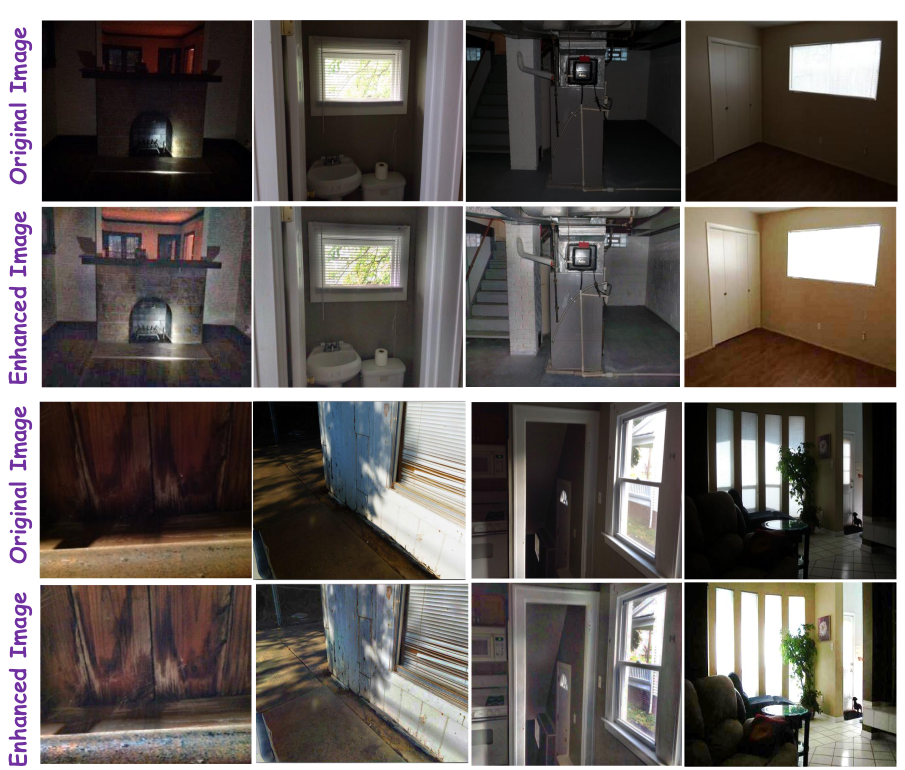
\includegraphics[width=1\linewidth, height=0.5\textheight]{images/lstm_clahe_example}
	\caption[Ejemplo aplicación del algoritmo C.L.A.H.E.]{Ejemplo aplicación del algoritmo C.L.A.H.E.}
	\label{fig:lstmclaheexample}
\end{figure}

La propuesta de estos investigadores se basa en aprender la información de la escena secuencialmente, tanto de forma vertical como horizontal. Para hacerlo, crearon dos redes recurrentes LSTM (Long Short Term Memory) con cuatro (4) capas ocultas de cientoveintiocho (128) unidades cada una. Como segundo punto, alimentan a la red con los datos de las imágenes de forma secuencial, es decir, transforman las imágenes a un tamaño de 128x128 y luego alimentan la red con la información secuencial de cada pixel de forma vertical para una de las redes y de forma horizontal para la otra. Para finalizar, introducen una capa densa totalmente conectada (fully connected layer, en inglés) con las salidas de ambas LSTM, seguida de otra capa densa totalmente conectada que concluye con una capa densa final con activación Softmax.

La arquitectura final propuesta como se puede observar en la Fig. \ref{fig:lstmarchitecture}, queda de la siguiente manera: dos redes LSTM que reciben los pixeles orientados de forma vertical y horizontal, respectivamente; una capa densa totalmente conectada que recibe las salidas de cada celda de la red LSTM, otra capa densa totalmente conectada que se concatena a la anterior y una capa densa final con activación Softmax que brinda las salidas.
Vale mencionar que es necesaria la aplicación del algoritmo CLAHE a cada imagen para el posterior entrenamiento y clasificación mediante la red propuesta.

\begin{figure}[h]
	\centering
	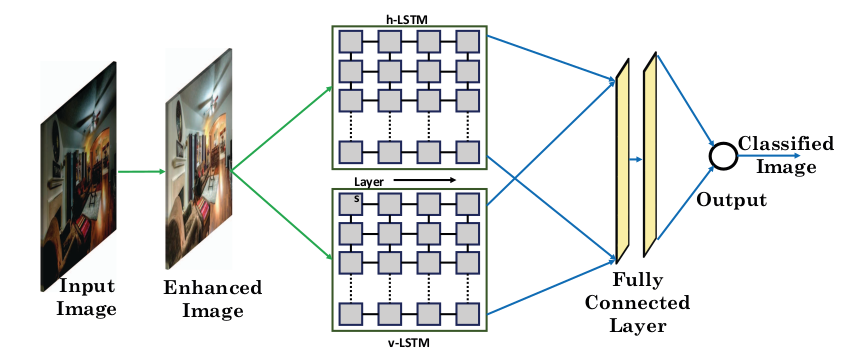
\includegraphics[width=1\linewidth,height=0.3\textheight]{images/lstm_architecture}
	\caption[Arquitectura de la red presentada]{Arquitectura de la red presentada}
	\label{fig:lstmarchitecture}
\end{figure}

Las comparaciones realizadas por los investigadores se basan en la métrica Exactitud (Accuracy, en inglés), se emplean utilizando diferentes configuraciones de esta red, y en relación al conjunto de datos propuesto por ellos (Real Estate Images, en inglés) además del conjunto de datos abierto \(SUN\). Los investigadores obtienen como mejores valores un 96.92\% de exactitud en el conjunto de datos propuesto \(REI\), y un 90.24\% en el la base de datos de imágenes \(SUN\), utilizando la configuación descripta anteriormente.
De esta manera quedan por encima de los resultados de utilizar extracción de características de redes preentrenadas con el conjunto de datos abiertos \(ImageNet\) con las arquitecturas AlexNet y VGGNet.

 

\subsection{Clasificación de escenas mediante Redes Neuronales Convolucionales}


En \cite{learning_deep_features} se creó una nueva base de datos con siete (7) millones de imágenes de escenas etiquetadas. Zhou y otros utilizaron Redes Neuronales Convolucionales para aprender características profundas sobre las escenas y alcanzar un nuevo estado del arte. Ellos se encargaron de mostrar que las características de más alto nivel aprendidas por redes neuronales profundas en conjuntos de datos centrados en objetos y a escenas son diferentes: imágenes de objetos no contienen la riqueza y diversidad de informaión visual que brindan las imágenes de escenas y ambientes para poder identificarlos.

Su trabajo comienza por la construcción del banco de imágenes: creación de URLs a partir de sustantivos y adjetivos relacionados a las escenas, eliminación de los links duplicados y luego de realizada la descarga, la eliminación de imágenes que se encuentren ya en el SUN database. Comparar la calidad del conjunto de datos generado en relación a otros de similar magnitud depende no sólo de las imágenes que contengan y sus categorías, sino también de múltiples factores como la variabilidad de las posiciones de la cámara, los estilos de decorado, la ubicación y el tamaño que los objetos ocupan dentro de la imagen, etc. Es razonable asumir que una buena base de datos de imágenes debería ser densa y diversa. La densidad de una medida de concentración de los datos, y una base de datos de imágenes debe serlo ya que para aprender sobre un elemento (en este caso escenas) es necesario que haya alto grado de concentración de ese elemento. La realidad es que la densidad de un conjunto de datos no alcanza, ya que si se cuenta con todas imágenes de la misma habitación tendrá una densidad muy alta pero una diversidad muy escaza. La diversidad es una medida relacionada a la cantidad de clases en un conjunto de datos; una base de datos de imágenes debe ser diversa porque es necesario que haya tanto múltiples elementos dentro de la misma como también variabilidad de enfoques para sus imágenes. Ambas medidas son difíciles de medir en conjuntos de datos de imágenes.
En este caso, los autores proponen dos medidas: densidad relativa y diversidad relativa. Para la primera los autores asumen que, en el dominio de las bases de datos de imágenes, una alta densidad es equivalente a que en general las imágenes tienen vecinos similares. Por esta razón para realizar la medición toman una imagen aleatoria de un conjunto de datos \(A\) (llámese \(a_{1}\)) y una imagen aleatoria del segundo conjunto de datos \(B\)  (llámese \(b_{1}\)). Si el conjunto \(A\) es más denso que el conjunto \(B\), entonces es más probable que \(a_{1}\) tenga menor distancia \(d\) a su vecino más cercano que \(b_{1}\), siendo \(d\) una medida de distancia entre dos imágenes en la que menores valores significa mayor similaridad. Con esta definición, se tiene que \(A\) es más denso que \(B\) si y sólo si la densidad de  \(A\) dado \(B\) es mayor que la densidad de \(B\) dado \(A\). 
\begin{equation}
{Den}_{B}(A)=p\left(d\left(a_{1}, a_{2}\right)<d\left(b_{1}, b_{2}\right)\right)
\end{equation}

Esta noción de densidad también puede aplicarse a múltiples conjuntos de datos \({A_{1}, \ldots, A_{N}}\):

\begin{equation}
{Den}_{A_{2}, \ldots, A_{N}}\left(A_{1}\right)=p\left(d\left(a_{11}, a_{12}\right)<\min _{i=2: N} d\left(a_{i 1}, a_{i 2}\right)\right)
\end{equation}

 Si de diversidad se trata, existen varias formas de medirla que mayormente se utilizan en biología para conocer la riqueza de un ecosistema. Para este trabajo los investigadores se basaron en el índice Simpson de diversidad que es una medida de qué tan bien están distribuidos los individuos de las diferentes especies en un ecosistema, y está relacionado a la entropía de la distribución de los mismos. Ellos proponen medir la diversidad relativa de dos conjuntos de datos \(A\) y \(B\) basándose en la idea de que \(A\) resultará más diverso si al selecionar aleatoriamente dos imágenes de \(B\) resultan más similares visualmente que seleccionar aleatoriamente dos imágenes de \(A\). De esta manera, la diversidad de \(A\) con respecto a \(B\) puede ser definida como:
 \begin{equation}
 {Div}_{B}(A)=1-p\left(d\left(a_{1}, a_{2}\right)<d\left(b_{1}, b_{2}\right)\right)
 \end{equation}
  donde \(a_{1}\) y \(a_{2}\) pertencen a \(A\) y  \(b_{1}\) y \(b_{2}\) pertenecen a \(B\) y fueron todas las imágenes seleccionadas aleatoriamente. De igual manera a la medida anterior, es posible de ser calculada entre más bases de datos de imágenes \({A_{1}, \ldots, A_{N}}\):
  
  \begin{equation}
  {Div}_{A_{2}, \ldots, A_{N}}\left(A_{1}\right)=1-p\left(d\left(a_{11}, a_{12}\right)<\min _{i=2: N} d\left(a_{i 1}, a_{i 2}\right)\right)
  \end{equation}
  
  siendo \(a_{i 1}, a_{i 2} \in A_{i}\) seleccionados aleatoriamente.
  
En el marco de la experimentación realizada para demostrar que las redes aprenden características diferentes según el tipo de conjunto de datos que se utilice para entrenarlas los investigadores se quedaron con aproximadamente 2.48 millones de imágenes correspondientes a 205 categorías con un mínimo de cinco mil y un máximo de quince mil imágenes por cada una como set de entrenamiento (al cual se refieren como "Places205"). El set de validación se seleccionó con cien imágenes por escena y el set de test doscientas, alcanzando un total de cuarenta y un mil imágenes entre estas dos últimas particiones. 
Finalizado el entrenamiento, los investigadores comparan las respuestas de unidades de varias capas de la red para entender mejor las diferencias entre ImageNet-CNN y Places-CNN, dos redes que tienen idéntica arquitectura pero que fueron entrenadas con conjuntos de datos de datos creados para diferentes propósitos (objetos y escenas, respectivamente). Las diferencias mayores entre las activaciones se dan a partir de la capa de pooling númuero dos gradualmente hasta la número cinco y también en la capa totalmente conectada número siete, en las que para ImageNet-CNN los campos receptivos se asemejan más a partes de objetos mientras que para Places-CNN en las mismas capas los campos receptivos parecen ser paisajes o estructuras relacionadas a un espacio. 
\begin{figure}[h!]
	\centering
	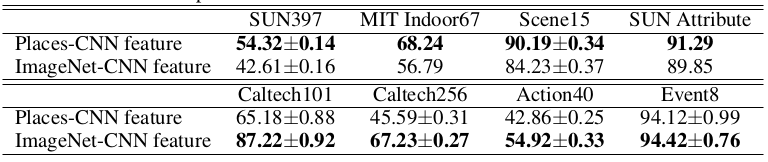
\includegraphics[width=1\linewidth]{images/places_metrics}
	\caption[Métricas por conjunto de datos y red]{Métricas por conjunto de datos y red}
	\label{fig:placesmetrics}
\end{figure}
En Fig. \ref{fig:placesmetrics} los investigadores hacen una comparación sobre conjuntos de imágenes tanto centradas en objetos como en escenas. La métrica utilizada es exactitud y las bases de datos de imágenes con que compararon fueron: SUN397, MIT INDOOR67, SCENE15, SUN Attribute, CALTECH101, CALTECH256, ACTION40, EVENT8. En los primeros cuatro, centrados a imágenes, los resultados obtenidos por Places-CNN son mayores a los de ImageNet-CNN. En los segundas cuatro bases de datos de imágenes, que son centradas en objetos, ImageNet-CNN obtiene mejores resultados. 


Para finalizar, entrenaron una red híbrida combinando el set de datos de entrenamiento de Places-CNN y de ImageNet-CNN. La llamaron Hybrid-CNN y luego de remover categorías solapadas alcanzó los 3.5 millones de imágenes pertenecientes a 1183 etiquetas diferentes. Esta red logró pequeñas mejoras en algunos de los conjuntos de datos utilizados en la comparación entre Places-CNN e ImageNet-CNN. Los resultados se muestran en Fig. \ref{fig:placesmetricshybrid}.
\begin{figure}[h!]
	\centering
	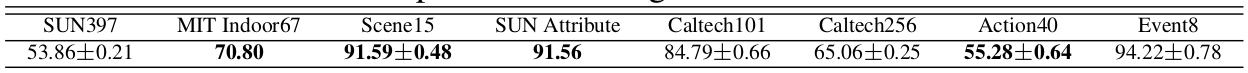
\includegraphics[width=1\linewidth]{images/places_metrics_hybrid}
	\caption[Métricas por conjunto de datos - Hybrid-CNN]{Métricas por conjunto de datos - Hybrid-CNN}
	\label{fig:placesmetricshybrid}
\end{figure}


En \cite{object_detectors_emerge_in_deep_scene_cnns} demostraron que no es necesario entrenar múltiples redes para realizar las tareas de clasificación de escenas y detección de objetos de una sola vez, ya que los detectores de objetos emergen por sí mismos en redes neuronales convolucionales entrenadas con bases de datos de escenas. 
Entender las representaciones aprendidas en las capas intermedias de arquitecturas profundas es un factor importante y del cual se podría sacar más provecho. Como las escenas están, en parte, compuestas por objetos, las redes neuronales convolucionales entrenadas para esta tarea aprenden a identificarlos internamente para definir de qué escena se trata, ergo la clasificación de escenas y la detección de objetos puede ser realizada en un mismo recorrido hacia adelante de la red, sin la necesidad de dar a la misma explícitamente la noción de objetos.
La contribución más importante en este trabajo fue demostrar que las redes entrenadas para detección de escenas, internamente aprenden a detectar los objetos relacionados a estas escenas; característica que hace a estas redes explotables para realizar otros propósitos sin la necesidad de tomarse todo el trabajo de crear, entrenar y refinar una red más con la que detectar los objetos que se contienen en estas escenas. En mayor medida, si la red fue entrenada con un conjunto de datos centrado en objetos. 
Para esta tarea los investigadores buscaron simplificar las imágenes de entrada para poder conocer cuáles eran las características de éstas que concentraban la mayor parte de la información que es utilizada por la red, es decir, aquellas en las que luego de ir quitando resto de características de la escena, la exactitud con la que se predecía se mantenía similar. En el primer intento de realizar esta tarea, para cada imagen, ellos realizaron una segmentación a partir de los bordes y regiones, removiendo subregiones diferentes de la siguiente manera: en cada iteración se remueve aquel segmento que produce el menor decrecimiento en la puntuación de clasificación, hasta que la escena sea clasificada incorrectamente. Al finalizar este primer enfoque obtuvieron una representación de la imagen que contiene la información mínima necesaria para que la red clasifique correctamente la escena. 
En un segundo intento basado en la hipótesis de que para la red Places-CNN existían objetos cruciales en el reconocimiento de escenas, generaron representaciones mínimas de las imágenes utilizando el conjunto de datos totalmente anotado SUN Database en cambio de realizar una segmentación automática. Para hacerlo realizaron el mismo procedimiento que en el primer enfoque para obtener estas representaciones con la diferencia que tomaron como verdaderos los segmentos provistos por la base de datos SUN. Vale denotar que para cada escena, son objetos los que usualmente forman parte de la representación mínima necesaria por la red, como es posible observar en la Fig. \ref{fig:objectsdetectorsemergeminrepresentationexamples}.
\begin{figure}[h!]
	\centering
	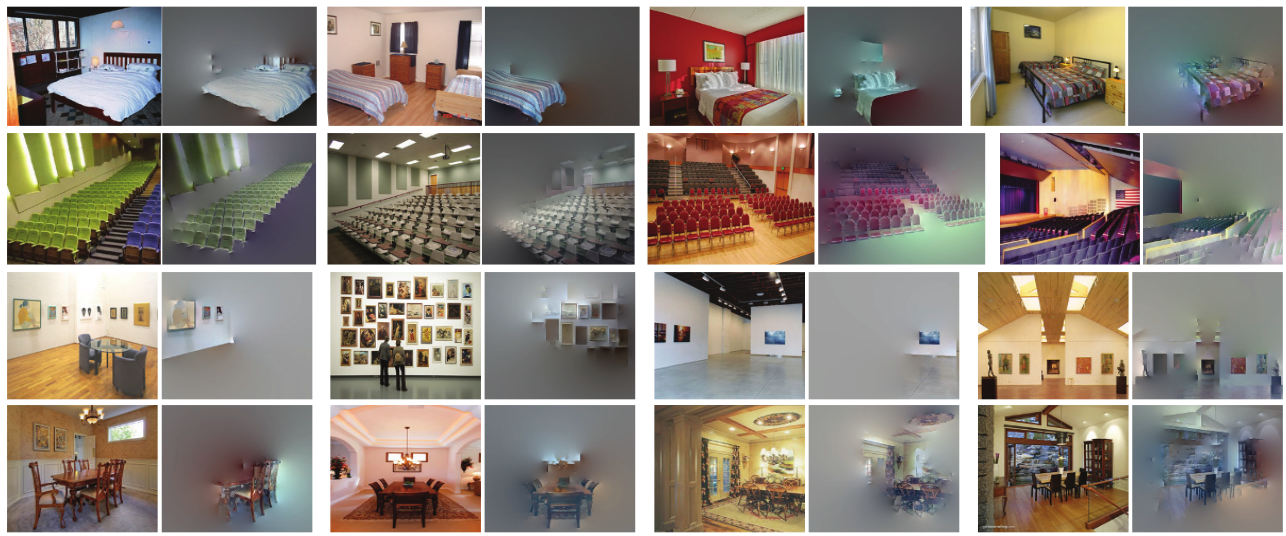
\includegraphics[width=1\linewidth]{images/objects_detectors_emerge_min_representation_examples}
	\caption[Ejemplos de representaciones mínimas encontradas]{Ejemplos de representaciones mínimas encontradas}
	\label{fig:objectsdetectorsemergeminrepresentationexamples}
\end{figure}

Para continuar con el trabajo, realizaron un análisis de los campos receptivos de las unidades y sus patrones de activación. Esto llevó a la observación de que las activaciones de las regiones tienden a tomar en mayor significado semántico a medida que se incrementa en la profundidad de las capas.
Finalmente, los investigadores brindan algunas razones de porqué emergen estos objetos en las tareas de clasificación de escenas: por un lado, que los objetos que emergen son los que más se encontraron en la base de datos SUN, por otro que éstos objetos que emergen son los que permiten discriminar mejor entre diferentes escenas, como es posible de observar en la Fig. 	\ref{fig:objectsdetectorsemergefinalexample}. Gracias a este trabajo es posible alcanzar el estado del arte en clasificación de escenas utilizando la red Places-CNN, pero también aprovechar las capas intermedias para encargarse de detectar los objetos que aparecen en estas escenas a partir de los campos receptivos de las mismas.
\begin{figure}[h!]
	\centering
	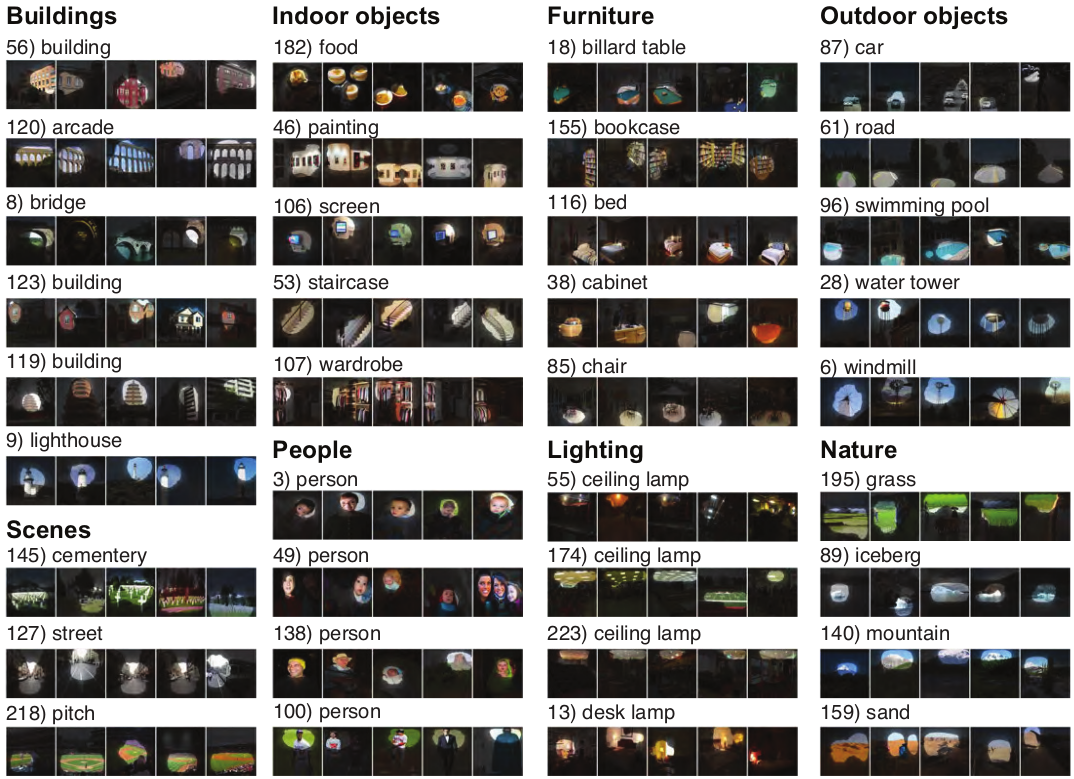
\includegraphics[width=1\linewidth, height=0.7\textheight]{images/objects_detectors_emerge_final_example}
	\caption[Ejemplos de objetos detectados a partir de la capa de pooling número 5]{Ejemplos de objetos detectados a partir de la capa de pooling número 5}
	\label{fig:objectsdetectorsemergefinalexample}
\end{figure}


En \cite{scene_recognition_cnn} Herranz y otros, basándose en la idea de que el reconocimiento de escenas requiere comprender tanto sobre escenas como de objetos en la escena, se dedicaron a la tarea de resolver dos problemas relacionados; por un lado el sesgo inducido por conjunto de datos relacionados a objetos de una escala en redes neuronales convolucionales entrenadas con objetos en múltiples escalas y por el otro, cómo combinar eficientemente el conocimiento obtenido de conjuntos de datos centrados en escenas y centrados en objetos.

En este trabajo ellos se encargaron de tener en cuenta la escala de los objetos para hacer que la red gane en razón de reconocimiento de las escenas. Para hacerlo eligieron centrarse en dos de los aspectos más importantes de las bases de datos de imágenes: escala y densidad. Por el lado de la escala, en el conjunto de datos ImageNet cada objeto ocupa casi el total de cada imagen, mientras que por el lado del conjunto de datos Sun397 los objetos son mucho más pequeños. Por parte de la densidad, en el conjunto de datos centrado en objetos, cada imagen contiene un gran objeto, mientras que en el centrado en escenas cada imagen contiene muchos objetos pequeños.

Gracias a la segmentación de objetos dentro de las escenas que lograron, fueron capaces de crear variaciones de un mismo elemento. De esta manera definieron y generaron los mismos objetos en dos escalas diferentes: escala original (la escala del objeto en la escena original) y escala canónica (se centra el objeto en la imagen y es reescalado para ocupar el tamaño de la imagen, manteniendo aspecto de radio).

La arquitectura propuesta por estos investigadores está enfocada a atender múltiples escalas mediante redes de escalas específicas. Esta gran red es una combinación de varias redes que operan en paralelo sobre sectores extraídos de la versión original de la imagen. Para cada una de las escalas utilizaron una red con una variante de la arquitectura AlexNetCNN llamada Caffe-Net. Para la extracción de los sectores, con el fin de acelerar el procesamiento, utilizaron una red totalmente convolucional (Fully convolutional network), con una capa de agrupamiento mediante máximos para agregar las características de los sectores en características de la imagen en sí.

Ellos detallaron sus dos diferencias principales con la arquitectura híbrida base. Primeramente, ellos utilizan el modelo más adecuado para cada escala de las imágenes. Luego, se encargaron de refinar individualmente los parámetros de cada uno de los modelos generados para adaptarse de la mejor manera a la escala. Además, remarcan que el punto de principal inflexión con el resto de trabajos similares es que ellos le dan importancia a la escala de la imagen, usando varias redes neuronales convolucionales en cambio de sólo una, alegando que las diferencias de escalas de los objetos entre las bases de datos ImageNet y Places dan lugar a la principal limitante de rendimiento.

La idea final que otorgan es que la información local obtenida de la capa totalmente conectada número 7 de la red ImageNet-CNN más la información global obtenida de la capa totalmente conectada número 7 de la red Places-CNN funciona mejor que la implementación híbrida base. Esto es así debido a que la red ImageNet-CNN aprende características sobre los objetos en sí (aprendizaje local), mientras que la red Places-CNN aprende características sobre las escenas completas (aprendizaje global).

En \cite{scene_classification_using_gbrcn} Zhang y otros dieron a conocer una nueva estructura para realizar esta tarea, con el cual sobrepasaron el estado del arte en los conjuntos de datos utilizados. Se trata de Redes Neuronales Convolucionales Aleatorias Potenciadas por el Gradiente (Gradient Boosting Random Convolutional Neural Network, su nomenclatura en inglés), una forma de aprendizaje conjunto (ensemble) que combina varias redes neuronales profundas.
Dentro de los aportes más significativos del trabajo se encuentran: la introducción de la red mencionada anteriormente en sí, una nueva función de pérdida multi-clase para poder combinar la potenciación por el gradiente con redes convolucionales y finalmente una variante a la red convolucional llamada red convolucional aleatoria (Random Convolutional Neural Network) que sirve como aprendiz base en tareas de aprendizaje conjunto profundo.
La red está diseñada para generar un ensamblado de redes convolucionales aleatorias (RCNet) de manera de poder combinarlas usando una función de pérdida que se ajusta a la red base. La red propuesta como bien se mencionó anteriormente es un ensamblado, es decir, de múltiples redes intentado minimizar la función de costo y mapear datos de entrada con una salida a través de la estimación de una función que sea capaz de realizar este mapeo, en este caso, esta función estará formada por un conjunto de \(M\) funciones agregadas de forma aditiva. 
\begin{equation}
\hat{f}(x)=\hat{f}^{M}(x)=\sum_{t=0}^{M} \hat{f}_{t}(x)
\end{equation}
Los autores proponen tanto una nueva red base como una función de pérdida para éstas. La función de costo está dada por:
\begin{equation}
\Psi(y, \hat{f}(x))=-\sum_{k=1}^{K} y_{k} \log p_{k}(x)
\end{equation}
donde la etiqueta a predecir está representada como 1 de los \(K\) vectores, siendo \(K\) igual al número de clases. \(f(x)\) es la estimación general de la función de ensamblado y \(p_{k}(x)\) es:
\begin{equation}
p_{k}(x)=\frac{\exp \left(f_{k}(x)\right)}{\sum_{l=1}^{K} \exp \left(f_{l}(x)\right)}
\end{equation}

Basándose en la aleatoriedad de los Bosques Aleatorios, con el fin de evitar el sobreentrenamiento por compartir todas las características entre todas las redes del ensamblado, los autores propuesieron una variante a las funciones CNet: RCNet, que aleatoriamente comparte algunos de los parametros con otras de las redes del ensamblado mediante un banco de filtros.

\begin{figure}[h]
	\centering
	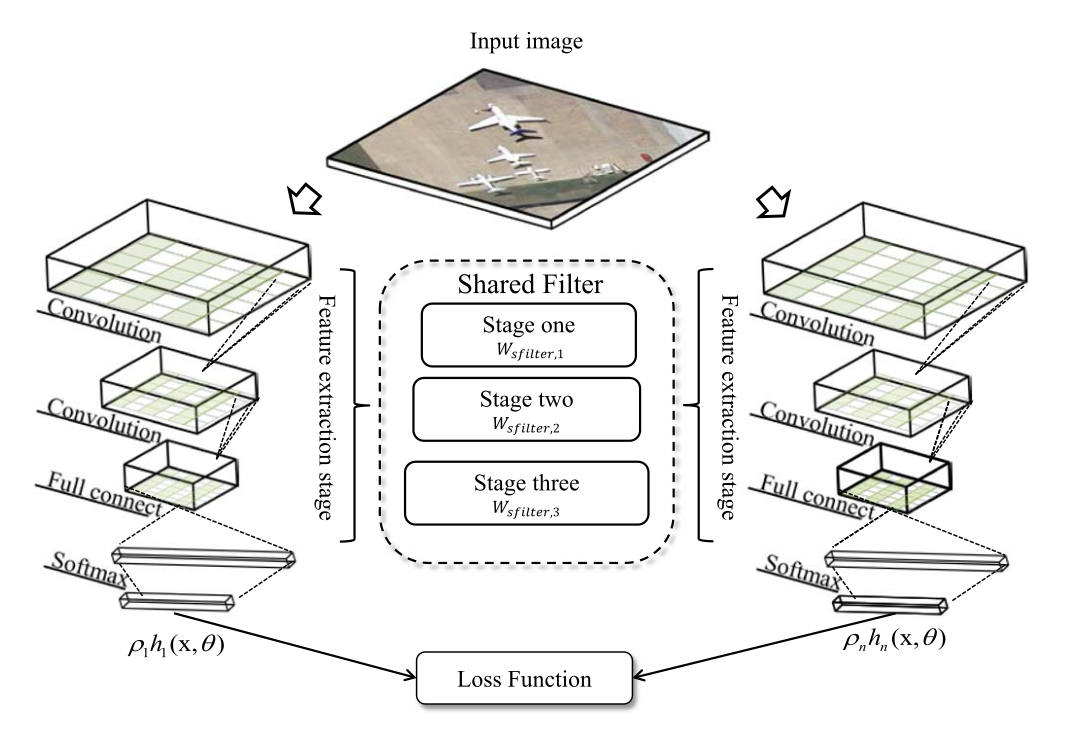
\includegraphics[width=1\linewidth]{images/gbrcnn_architecture}
	\caption[Arquitectura de la red]{Arquitectura de la red}
	\label{fig:gbrcnnarchitecture}
\end{figure}


Durante cada función RCNet se muestrea aleatoriamente un set de filtros del banco de filtros compartidos para construir la etapa de extración de características de la RCNet y simultáneamente actualizar los parámetros de la RCNet y el banco de filtros compartido. El tamaño del filtro del banco de filtros compartidos es mayor al del filtro en la función RCNet de manera que diferentes redes compartirán algunos parámetros. 

Para concluir, los investigadores pusieron a prueba la arquitectura (ver Fig. \ref{fig:gbrcnnarchitecture}) con dos conjuntos de datos centrados en imágenes satelitales, comparando los resultados con arquitecturas clásicas de clasificación de imágenes y demostrando no sólo que la red propuesta es apropiada como aprendiz base en arquitecturas de ensamblado, sino que también es posible alcanzar el estado del arte y superarlos en relación a los métodos tradicionales.

\subsection{Clasificación de escenas mediante Aprendizaje por Transferencia} \label{ssec:transfer_learning}
En \cite{raahlen2019image}, un trabajo realizado por R{\aa}hl{\'e}n Oskar y Sj{\"o}qvist Sacharias en 2019, se trabajó específicamente con los fines de utilizar el aprendizaje mediante transferencia para clasificar imágenes de propiedades.
Resumidamente, ya que luego se abordará debidamente el tópico en el marco teórico, el aprendizaje mediante transferencia se trata de utilizar una red preentrenada \(R\) con un conjunto de datos \(A\) para resolver un problema relacionado a un conjunto de datos \(B\), y la manera para hacerlo es reentrenar la red \(R\) con los datos del conjunto de datos \(B\). Para este proyecto utilizaron como redes preentrenadas ResNet18, AlexNet, VGG-11, DenseNet-121 e Inception-v3.
Los datos con los que cuentan en esta investigación son imágenes extraídas de Google Image search y \cite{hemnet}, distribuidos de la siguiente manera para cada etiqueta como se observa en la Fig. \ref{fig:transferlearningdataset}.
\begin{figure}[h!]
	\centering
	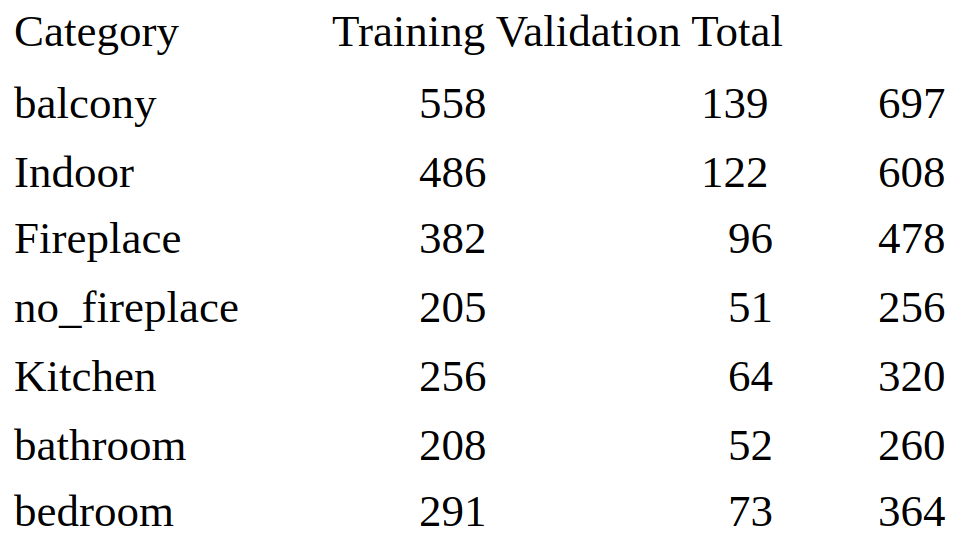
\includegraphics[width=0.7\linewidth]{images/transfer_learning_dataset}
	\caption[Distribución de las imágenes por categoría etiquetada]{Distribución de las imágenes por categoría etiquetada}
	\label{fig:transferlearningdataset}
\end{figure}


En el trabajo se realizaron tres experimentos, y en cada uno de ellos se testearon todas las redes descriptas previamente, con y sin refinamiento de las mismas. El primero se trata de un clasificador binario para predecir si una imagen contiene o no un balcón; el segundo es igualmente un clasificador binario pero que predice si en la imagen se encuentra un hogar (por ejemplo, hogar a leña), y en el tercer experimento plantean una clasificación multiclase en la que intentan etiquetar las imágenes según si se trata de una cocina, un dormitorio o un baño. Es sobre éste último en el cual se hará énfasis. 
Los primeros dos experimentos con clasificadores binarios no resultan de gran interés para este problema, aunque es importante remarcar que para el primero se alcanza una exactitud de un 98\% luego de refinamientos utilizando la red Inception-v3, mientras que para el segundo el mayor porcentaje se alcanza con la red DenseNet y alcanza un 85.5\%. 
El experimento realizado que resulta de mayor importancia para este proyecto es el tercero, un clasificador de múltiples etiquetas que intenta determinar si la imagen se trata de una cocina, un dormitorio o un baño. Las métricas obtenidas antes de realizar refinamiento de las redes testeadas se dan a conocer en la Fig. \ref{fig:metricstransferlearning}
\begin{figure}[h!]
	\centering
	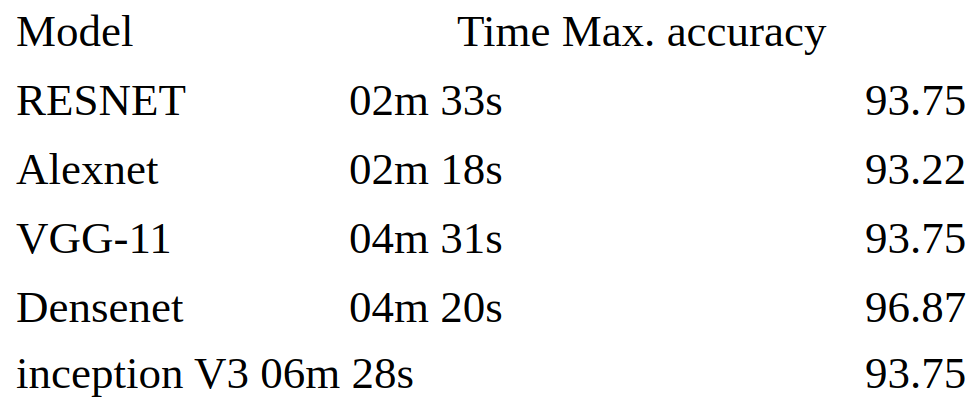
\includegraphics[width=0.6\linewidth]{images/metrics_transfer_learning}
	\caption[metrics_transfer_learning]{Métricas usando extracción de características de los modelos preentrenados}
	\label{fig:metricstransferlearning}
\end{figure}
Luego de hacer refinamiento de las redes entrenando con las imágenes del conjunto de datos generado por los investigadores se alcanzan los resultados expuestos en la Fig \ref{fig:metricstransferlearningfinetunned}.

\begin{figure}[h!]
	\centering
	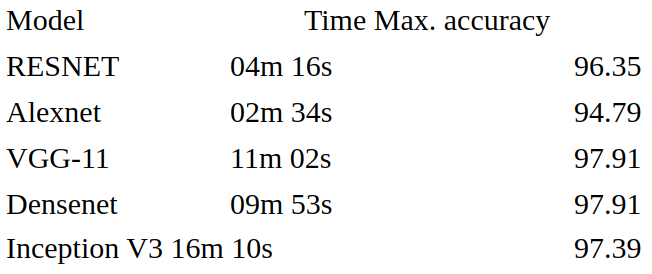
\includegraphics[width=0.7\linewidth]{images/metrics_transfer_learning_fine_tunned}
	\caption[metricstransferlearningfinetunned]{Métricas luego de realizar refinamiento de las redes}
	\label{fig:metricstransferlearningfinetunned}
\end{figure}

Como se puede observar, luego de reentrenar los modelos se obtienen mejoras representativas, dado el percentil de exactitud en que se encuentran los resultados. Otro punto a denotar es que en ambos casos es la red DenseNet la que obtiene la mejor performance, aunque toma aproximadamente el doble de tiempo que el resto de las redes en entrenarse.
Los autores concluyen su trabajo explicando que a partir de un bajo número de imágenes en su conjunto de datos, y a través de aprendizaje por transferencia, es posible agregar palabras claves a las imágenes, como ser: balcón, hogar, baño, cocina y habitación.

\subsection{Otros trabajos relacionados a las propiedades inmuebles que toman provecho de las imágenes de los mismos}

En \cite{vision_based_real_estate_price_estimation} Poursaeed y otros se dedican a la tarea de la estimación de precios de inmuebles basándose en las características visuales de las propiedades. El trabajo incluye una evaluación del impacto visual de las características de una casa en su valor de mercado, la estimación de lujosidad mediante redes neuronales convolucionales, un armazón para la automatización de la valuación utilizando tanto imágenes de las propiedades como metadatos de las mismas y experimentos en los que aplican su trabajo a un nuevo conjunto de datos.
Para comenzar se encargaron de obtener alrededor de doscientas mil imágenes correspondientes a diferentes ambientes de casas a partir del conjunto de datos Places, Houzz (una empresa de alquiler y venta de viviendas) y búsquedas en Google Imágenes. Luego, entrenaron una red con arquitectura DenseNet para la tarea de predecir las etiquetas baño, dormitorio, cocina, living, comedor, interior y exterior. Con este clasificador, alcanzaron un 91\% de exactitud en el conjunto de validación.
\begin{figure}
	\centering
	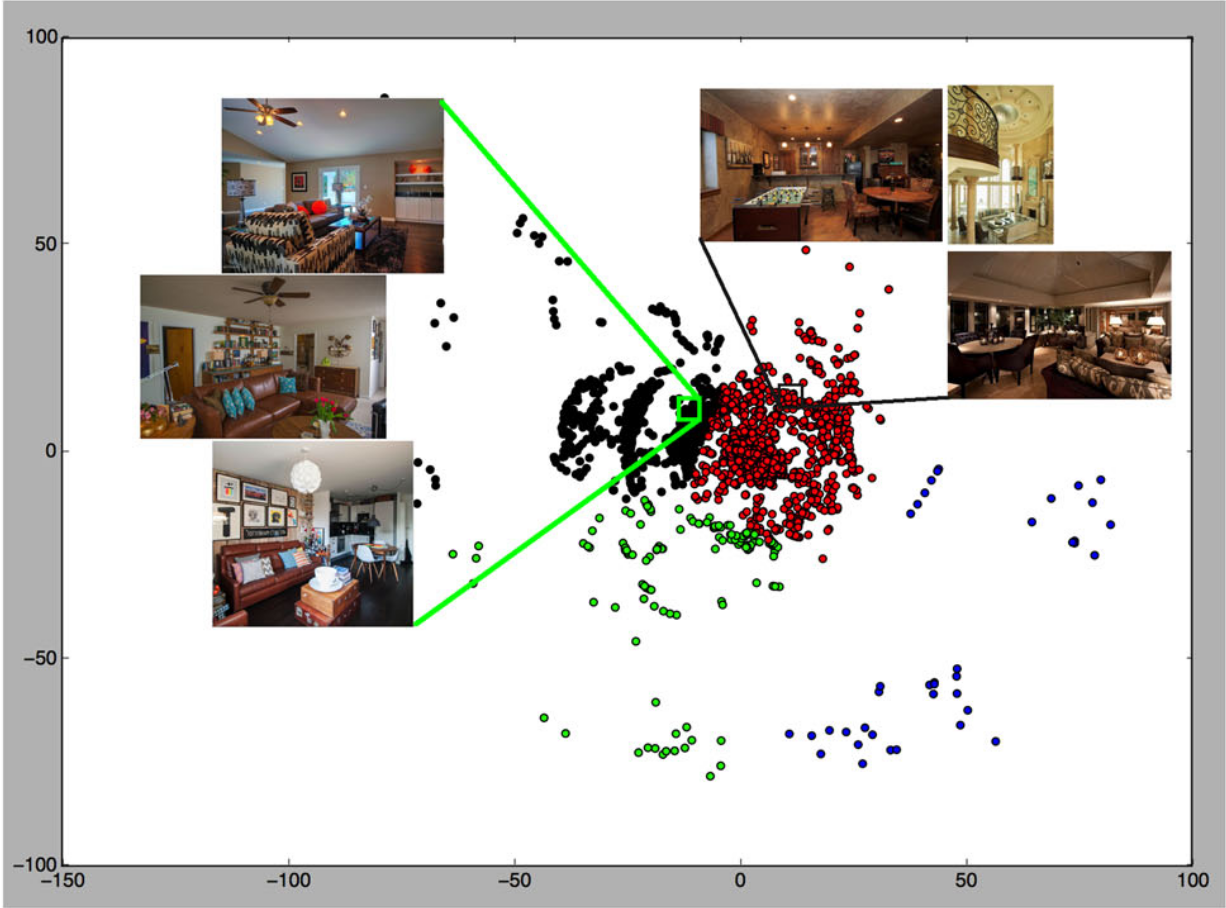
\includegraphics[width=0.9\linewidth]{images/vision_based_example_3c}
	\caption[Figura 3.c de Vision Based Real Estate Price Estimation]{Figura 3.c de Vision Based Real Estate Price Estimation}
	\label{fig:visionbasedexample3c}
\end{figure}

A partir de las imágenes etiquedas, en esta investigación propusieron segmentar cada habitación en ocho niveles de lujosidad utilizando la herramienta de crowdsourcing Amazon Mechanical Turk con el fin de obtener estas etiquetas de cada sector. De esta manera, se hicieron de un embedding (descripto en \ref{embedding}) de baja dimensión en el cual las imágenes con el mismo nivel de lujosidad se encuentran cercanas entre sí, como se puede ver en la figura \ref{fig:vision_based_example_3c}, extraída de la figura \(3.c\) de \cite{vision_based_real_estate_price_estimation}. Mediante el algoritmo t-STE los investigadores obtuvieron un embedding bidimensional de las imágenes, que a partir de visualizaciones de los clusters se determinó que las imágenes con mayor nivel de lujosidad quedan en el centro, mientras que las menos lujosas se ubican alrededor. Para aquellas casas que no presentaban imagen de alguno de los ambientes, lo que hicieron fue imputar el promedio de las otras categorías para representar el nivel de lujosidad de ese ambiente.
Una actividad aparte para ellos fue la estimación de precios, para la cual implementaron una regresión que absorve tanto la salida de los modelos que estiman la lujosidad de las habitaciones previamente clasificadas por la DenseNet, como metadatos al respecto de la propiedad (precio de oferta, tamaño, años desde su construcción, cantidad de habitaciones de cada tipo, etc). Vale aclarar que la etiqueta a predecir en cada propiedad es el valor final al que fue adquirida.
\begin{figure}[h!]
	\centering
	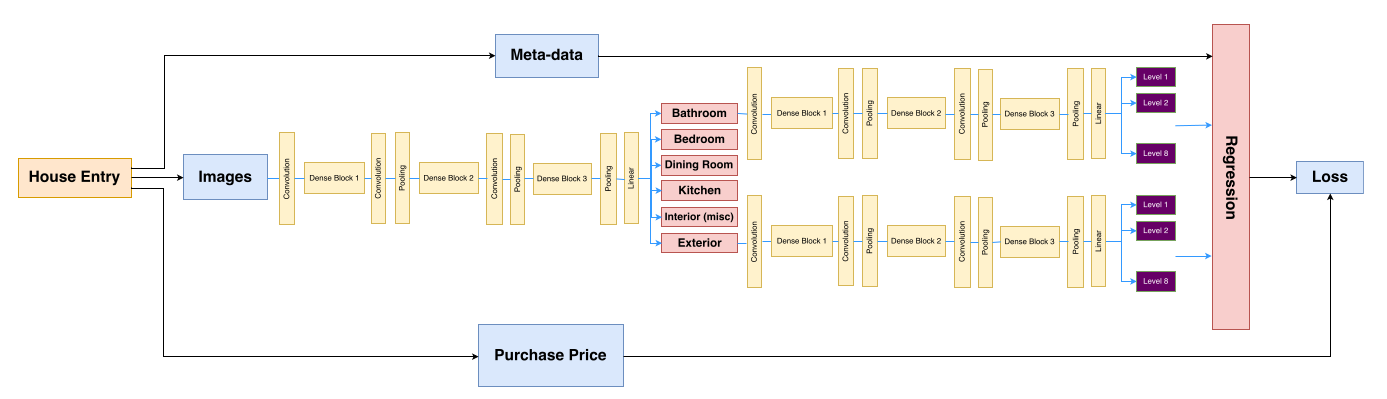
\includegraphics[width=1\linewidth, height=0.35\textheight]{arquitectura_vision_based}
	\caption[Vision Based Architecture]{Arquitectura de la red descripta}
	\label{fig:arquitecturavisionbased}
\end{figure}

Finalmente, con la arquitectura utilizada (ver Fig. 	\ref{fig:arquitecturavisionbased}) demostraron que es posible mejorar los resultados de estimaciones que actualmente se utilizan en el mercado (Índice Zestimate de Zillow) disminuyendo la mediana del error de un 7.9\% a un 5.6\% logrado a partir de la arquitectura presentada.

\subsection{Antecedentes no académicos}
Dentro de los antecedentes que no califican como investigaciones, nos encontramos con \(Restb AI\) \cite{restb_ai}, una empresa que comenzó en 2016 de la mano de Angel Esteban. "Buscando entre docenas de propiedades, él estaba shockeado por la inconsistencia en la calidad de las mismas y la dificultad general para encontrar la casa de ensueños para su familia. Tenía que haber una mejor manera." es lo que muestran en la historia de la empresa, que actualmente cuenta con oficinas en Estados Unidos y Europa.
Dentro de las capacidades de visión por computadora que listan relacionadas a las propiedades se encuentran la clasificación de escenas, la detección de características dentro de una imagen, análisis de estado de las habitaciones.
Además, gracias a las capacidades mencionadas anteriormente en su sitio, demuestran cómo se aprovecharon del etiquetado de las imágenes para generar sus productos. Éstos son avocados a la experiencia de usuario, modelos de datos y moderación de contenido. En relación a la experiencia de usuario detallan tres productos fundamentales: la experiencia en búsquedas, el análisis comparativo del mercado y la conversión de imagen a discurso. Por el lado de los modelos de datos se encuentran la valoración automática de propiedades, completar información al respecto de una propiedad que pueda no haber sido detallada, es decir, la integridad de datos, las publicidades dirigidas y la análitica de datos relacionados a este contexto. Por parte de la moderación de contenidos se encuentra la detección de marcas de agua, detección de imágenes duplicadas y la detección de información sensible dentro de la imagen (patentes, números telefónicos, rostros).
Como se puede ver, algunos de estos productos resultan ya definidos como posibles formas de aprovechar el etiquetado de imágenes en la motivación del proyecto, aunque otros no fueron mencionados y también continúan agregando valor y razón de ser a esta investigación.
\vfill

\section{Marco teórico}
\subsection{Aprendizaje automático}
%- explicación resumida tipos de aprendizaje (supervisado, no supervisado, semisupervisado)
 Dentro de las diferentes ramas de la inteligencia artificial, los algoritmos utilizados se pueden clasificar en tres grandes ramas según la forma en que son entrenados: algoritmos de aprendizaje supervisado, algoritmos de aprendizaje semi-supervisado y algoritmos de aprendizaje no supervisado. Los primeros son los que se utilizan cuando para el conjunto de entrenamiento \(X\) se tiene un conjunto de etiquetas \(y\) con las que se relacionan unívocamente, y de esta manera, los algoritmos encuadrados dentro de esta rama se encargan de estimar una función que mapee los datos del conjunto \(X\) al conjunto \(y\), con el fin de  luego poder realizar inferencias a partir de sólo nuevos casos de entrada. Los algoritmos de aprendizaje no supervisado se utilizan en situaciones en las que se tiene un conjunto de datos de entrada \(X\) pero no se tiene un conjunto de etiquetas asignadas a estos datos, estos algoritmos se emplean para realizar sobre los datos tareas tales como agrupamientos, detección de anomalías, reducción de dimensionalidad, entre otras. Por último, la rama del aprendizaje semi-supervisado entra en juego para aquellos casos en los que se tiene un pequeño conjunto de datos etiquetado, y un gran conjunto de datos no etiquetados.
 
%- explicación profunda aprendizaje supervisado, ejemplos otros tipos de problemas
 En este trabajo se contará tanto con un conjunto de entrenamiento que serán bases de datos de imágenes como con sus pertenecientes etiquetas, por lo que se intentará mapear mediante algún algoritmo (en este caso técnicas de aprendizaje profundo) cada imagen con sus etiquetas: aprendizaje supervisado.
 
 Dentro de esta rama existen otros algoritmos que pueden servir para este problema o para otros problemas de dominio diferente como son los árboles de decisión, regresiones lineales o logísticas, ensembles, etc.
 
\subsection{Representación de una neurona}
%- explicación neurona
 En este trabajo, como bien se explicó anteriormente, se abordará la solución mediante técnicas de aprendizaje profundo, por lo que a continuación se dara lugar a las explicaciones pertinentes relacionadas a este tipo de técnica.
 Para empezar es necesario comentar que el término "profundo" recae en la profundidad de las redes neuronales que se utilizan en esta técnica. Estas redes pueden estar compuestas hasta por millones de neuronas interconectadas entre si; neuronas que se representan como se observa en la imagen \ref{fig:representacion_neurona} en donde se muestra un ejemplo de una neurona con \(n\) entradas, conformada por: 
 \begin{itemize}
 	\item Entradas: conjunto de datos de entrada \(x_1\)..\(x_n\)
 	\item Pesos: conjunto de pesos \(w_1\)..\(w_n\) correspondientes a cada entrada
 	\item Función de agregación: función que agrega la multiplicación pesada entre cada entrada \(x\) y su correspondiente peso \(w\).
	\item Función de activación: función no lineal responsable de mapear el resultado de la función de agregación en salidas (según que tipo de función los resultados son valores entre [0, 1]o [-1, 1]).
	\item Salida: resultado de la función de activación.
 \end{itemize}
 
 
\begin{figure}
\centering
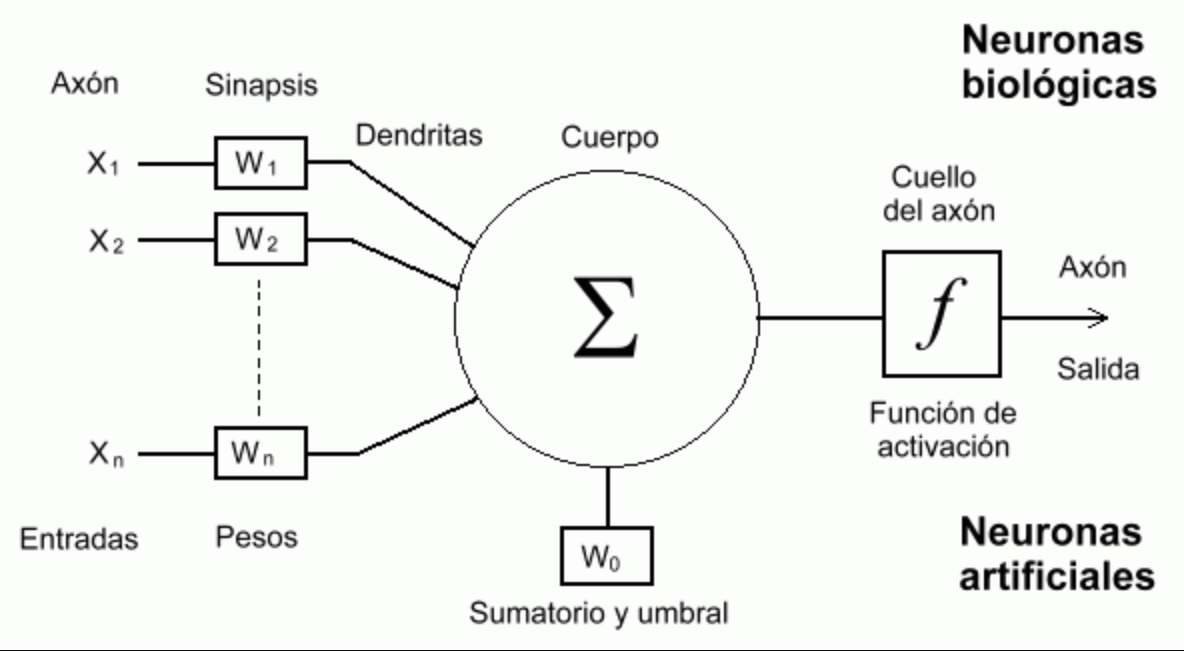
\includegraphics[width=0.7\linewidth]{images/representacion_neurona}
\caption[Representación de una neurona]{Representación de una neurona}
\label{fig:representacion_neurona}
\end{figure}

De esta manera, se puede obtener la salida de la neurona \(Y\), a partir de aplicar la función de activación \(\sigma\) a la suma entre el sesgo \(b\) y la multiplicación matricial del conjunto de entrenamiento \(X\) y los pesos \(W\).

\begin{equation}
Y=\sigma\left(W^{T} X^{(i)}+b\right)
\end{equation}


\subsection{Red Neuronal}

%- explicación redes neuronales profundas
 Una red neuronal, como su nombre lo enuncia, es una consecución de capas de \(N\) neuronas en cada una, conectadas entre sí como se puede ver en el ejemplo de la figura \ref{fig:redneuronal}. Es necesario que se cuente con capas de entrada, capas ocultas y capas de salida; para la figura \ref{fig:redneuronal} se tiene una capa de entrada, dos capas ocultas y una capa de salida. 
 El fin de las redes neuronales es aprender representaciones del contenido de la información en relación a las salidas esperadas para luego poder hacer inferencias en nuevo contenido, a modo de ejemplo, si se tienen imágenes de perros y gatos, y el fin es detectar si se trata de un perro o un gato la red posiblemente no aprenda las mismas representaciones que si el fin de la misma es detectar presencia o ausencia de animales.
 
 
 
 \begin{figure}
 	\centering
 	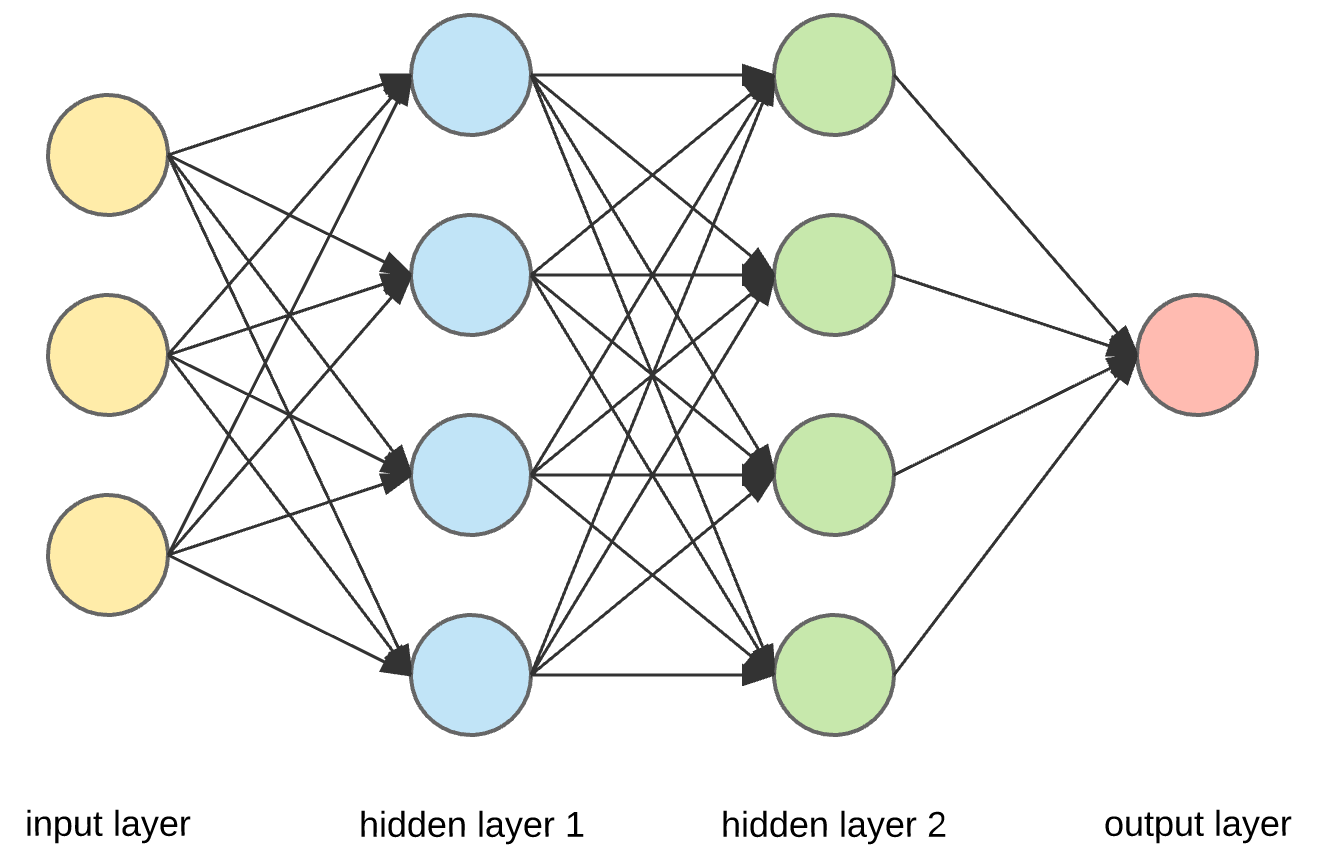
\includegraphics[width=0.7\linewidth]{images/red_neuronal}
 	\caption[Ejemplo red neuronal]{Perceptrón Multi Capa}
 	\label{fig:redneuronal}
 \end{figure}

 Para explicar el funcionamiento de las redes neuronales es necesario también introducir algunos conceptos como son la propagación hacia adelante y hacia atrás, función de pérdida y optimización. Durante la fase de entrenamiento, los pasos que se siguen son:
 \begin{enumerate}
 	\item Propagación hacia adelante
 	\item Evaluación de función de pérdida
 	\item Propagación hacia atrás
 \end{enumerate}
 La propagación hacia adelante es la actividad en la que se le brindan los datos a la capa de entrada de la red para que se evalúen todas las capas en esa dirección aplicando \ref{formula:forward_prop} en cada capa tomando como entrada la capa inmediata anterior. De esta manera, se obtiene como salida de la red sus predicciones. Luego, a partir de estos resultados es posible medir la función de pérdida, a partir de la cual se realiza la propagación hacia atrás del error.
  
 \begin{equation}\label{formula:forward_prop}
 z=W^{\wedge} T x+b
 \end{equation}
 


- explicacion funcionamiento:
	- forward prop 
	- back prop
	- regularizers:
		- dropout
		- batch norm
	- optimizers
	- metrics
	- loss functions
	
\subsection{Red Neuronal Convolucional}
- explicación razón de convoluciones
- partes:
	- Convolución
	- stride
	- pooling layers
- ejemplo simple

\subsection{Redes preentrenadas} 
- Transfer Learning
- Arquitecturas de las redes y datasets ejemplos

\subsection{Representación del conocimiento}
- Ejemplos activaciones
\vfill

\section{Diseño experimental}
\subsection{Asunciones}
En este trabajo se tomarán como ciertos los siguientes puntos:
\begin{enumerate}
	\item Los conjuntos de datos elegidos se encuetran etiquetados correctamente 
	\item Cada imagen de los conjuntos de datos con los que se entrenarán los modelos resultan representativas a la escena a la que pertenecen.
	\item El hardware con el que se llevará a cabo el proyecto funcionará tal y como se establece en sus respectivo manual.
	\item Las red preentrenada a descargar (PlacesCNN) fue entrenada sólo con las imágenes del conjuntos de datos Places.
	\item Para ambientes productivos la métrica \cite{balanced_accuracy_score} es la más representativa.
\end{enumerate}

\subsection{Limitaciones} \label{ssec:limitaciones}
El proyecto en curso contará con las siguientes limitaciones:
\begin{enumerate}
	\item El análisis se centrará en imágenes de las siguientes escenas de propiedades: cocina, comedor, baño, dormitorio, exterior, living, otros interior.
	\item Tanto los tiempos de entrenamiento y predicción como el tamaño de las redes, estarán restringidos al hardware con el que se cuenta.
	\item El trabajo intentará aceptar o refutar las hipótesis enumeradas a continuación, quedando excluídas del alcance del proyecto las posibles investigaciones que surjan a partir del mismo.
\end{enumerate}

\subsection{Hardware a utilizar} \label{ssec:hardware}
Para llevar adelante el trabajo se utilizarán los siguientes componentes:
\begin{itemize}
	\item Procesador Intel i7 de séptima generación versión U.
	\item Memoria RAM de 16gb.
	\item Disco sólido 256GB NVMe™ M.2 SSD.
	\item Tarjeta gráfica Gigabyte GTX 1080 de 8gb.
\end{itemize}

\subsection{Hipótesis}
Teniendo en cuenta tanto las limitaciones como las asunciones definidas para el trabajo, se comprobarán las hipótesis declaradas a continuación. 

\subsubsection{Hipótesis 1} \label{sssec:hipotesis1}
Como se pudo observar en la revisión de antecedentes, existen múltiples formas de hacer frente al problema. El enfoque más simple podría ser mediante perceptrón multicapa, pero por lo que se pudo observar, la mayoría de las soluciones utilizadas son redes neuronales convolucionales. Este punto de partida abre la primer hipótesis del trabajo: una red convolucional es capaz de obtener mejores resultados que un perceptrón multicapa en materia de clasificación de escenas.

\subsubsection{Hipótesis 2} \label{sssec:hipotesis2}
Las redes convolucionales tienen la capacidad de aprender características de las imágenes con las que se entrenan, aunque a veces resulta muy costoso hacerlo por las diferencias entre imágenes de la misma categoría o bien no se cuenta con la cantidad de imágenes que aporten la densidad y diversidad necesaria para alcanzar el tope máximo en la métrica elegida. 

Hipótesis: "Una red convolucional obtendrá mejores resultados sobre un conjunto de test \(y\) siendo entrenada con conjunto de entrenamiento \(X\) que si es entrenada sólo con subconjuntos de 10\% o 50\% del conjunto de entrenamiento \(X\), respectivamente".

%\subsubsection{Hipótesis 3} \label{sssec:hipotesis3}
%Dado que la cantidad de escenas a clasificar es relativamente baja, sería posible plantear un enfoque en el que se entrene una red convolucional para cada una de las mismas. En este caso se trataría de clasificación binaria en la que la red sea capaz de detectar si se trata de una escena o no, aunque se debería tener en consideración el hecho de no estar cometiendo sobreentrenamiento. La hipótesis a analizar en este punto es: \(N\) redes convolucionales entrenadas como clasificadores binarios (una para cada escena) mejoran los resultados que utilizar una sola red convolucional para clasificar las mismas \(N\) clases, es decir, los resultados obtenidos de contrastar la hipótesis \ref{sssec:hipotesis2}.

\subsubsection{Hipótesis 3} \label{sssec:hipotesis3}
Como se pudo ver en \cite{learning_deep_features}, Zhou y otros crearon una red entrenada con millones de imágenes de escenas (Places Dataset) que debería ser capaz de predecir las imágenes de las escenas con las que fue entrenada. En términos de cantidad de imágenes, esta red está mucho más entrenada que las utilizadas en este trabajo. 

Hipótesis: "Realizar inferencia directamente a partir de esta red preentrenada alcanza mejores resultados que una red convolucional entrenada con el conjunto de datos del trabajo \cite{vision_based_real_estate_price_estimation} (el de mayor cantidad de imágenes que se tiene) para los conjuntos de validación y verificación definidos al contrastar la hipótesis \ref{sssec:hipotesis2}".

\subsubsection{Hipótesis 4} \label{sssec:hipotesis4}
Una de las técnicas revisadas antes de comenzar con el trabajo es Aprendizaje por Transferencia (\ref{ssec:transfer_learning}), en el cual se parte de redes preentrenadas y se las reentrena con el conjunto de imágenes propio para ajustar los pesos al mismo. 

Hipótesis: "Haciendo aprendizaje por transferencia a partir de la red PlacesCNN es posible mejorar los resultados obtenidos al contrastar la hipótesis \ref{sssec:hipotesis3}".

\subsubsection{Hipótesis 5} \label{sssec:hipotesis5}
El Aprendizaje por Transferencia depende en gran medida del conjunto de datos utilizado al entrenar la red. Como se explicó en la revisión de antecedentes, ImageNet es una base de datos de imágenes centrada en objetos, mientras que el conjunto de datos Places es centrado en escenas. 

Hipótesis: "Una red pre-entrenada con imágenes centradas a escenas y con ajuste fino utilizando un conjunto de datos \(X\) consigue mejores resultados una red pre-entrenada con imágenes centradas a objetos y luego ajustada finamente mediante el mismo conjunto de datos \(X\)".

\subsection{Experimentos}
%Se validará cada hipótesis a partir de experimentos individuales con el fin de constratar cada una. 
Los conjuntos de datos a utilizar en los experimentos serán los generados en los trabajos \cite{vision_based_real_estate_price_estimation} y \cite{lstm_real_estate}, de los cuales se seleccionarán las escenas determinadas en las limitaciones del trabajo. En las tablas \ref{exp:distribution_rei} y \ref{exp:distribution_vision_based} se puede observar la distribución de escenas que contienen de los mismos. La métrica con la que se compararán los diferentes resultados será Precisión Categórica.

\begin{table}[h!]
	\centering
	\begin{tabular}{| l | r | }
		\toprule
		Escena &  Cantidad de imagenes \\
		\midrule
		backyard &       745 \\
		bathroom &       793 \\
		bedroom &      1593 \\
		frontyard &       884 \\
		kitchen &       992 \\
		living\_room &       852 \\
		\bottomrule
	\end{tabular}
	\caption{Imágenes por escena - Conjunto de datos del trabajo \cite{lstm_real_estate}}
	\label{exp:distribution_rei}
\end{table}

\begin{table}[h!]
	\centering
	\begin{tabular}{| l | r | }
		\toprule
		Escena &  Cantidad de imágenes \\
		\midrule
		bathroom & 10058 \\
		bedroom & 24123 \\
		dining\_room & 19500 \\
		frontyard & 24869 \\
		kitchen & 24234 \\
		living\_room & 24210 \\
		\bottomrule
	\end{tabular}
	\caption{Imágenes por escena - 	Conjunto de datos del trabajo \cite{vision_based_real_estate_price_estimation}}
	\label{exp:distribution_vision_based}
\end{table}

\subsubsection{Experimento 1} \label{sssec:exp1}
Se entranará tanto una red convolucional como un perceptrón multicapa con las imágenes del conjunto de datos generado en el trabajo \cite{vision_based_real_estate_price_estimation}. A continuación podremos comparar los resultados de ambos modelos de manera que será posible contrastarlos con la hipótesis \ref{sssec:hipotesis1}.

El perceptrón multicapa del experimento cuenta con cinco capas ocultas totalmente conectadas de 1024, 1024, 512, 256 y 128 neuronas en cada una, con una capa de dropout intercalada luego de cada una de ellas con probabilidad de 0.3, finalmente, una capa de salida con activación softmax como se observa en la imagen \ref{fig:h1mlpmodel}. 


Por el lado de la red neuronal convolucional se utilizará una arquitectura que concatenará dos bloques compuestos por: capa convolucional, capa de normalización en lote, capa convolucional, capa de normalización en lote, capa de pooling y capa de dropout; en el primer bloque las capas convolutivas aplicarán 64 filtros cada una, mientras que en el segundo 128, todos ellos de tamaño \([5\;x\;5]\) en todas las capas convolutivas, las capas de pooling aplicarán filtros de \([2\;x\;2]\) y las capas de dropout tendrán asignada una probabilidad de 0.25. Luego de estos bloques, la red seguirá con una capa totalmente conectada de 512 neuronas con regularización L2, una capa dropout con probabilidad 0.5 y la capa de salida con activación Softmax. La inicialización de los pesos de la red se realizará mediante inicialización de Xavier \cite{glorot2010understanding}. 

En ambas redes se utilizaron de la misma manera las siguientes configuraciones: 
\begin{itemize}
	\item Tamaño del lote: la cantidad de imágenes a computar antes de realizar una actualización de pesos es de 64.
	\item Entradas: ambas redes se entrenaron con los tres canales de las imágenes (Red, Green, Blue), redimensionando cada una a \(128\; x\; 128\) y luego normalizando el valor de los colores (se divide el valor de cada pixel sobre 255, el valor máximo en la escala RGB).
	\item Optimizador: exactitud categórica. En cada lote contabiliza las veces en las que la posición de la probabilidad más alta se condice con la posición de la predicción correcta. Vale aclarar que los resultados, al utilizar una capa de activación softmax son \(one-hot\; encoders\), es decir, para cada imagen se tiene como resultado un vector de longitud igual a la cantidad de clases a predecir con la probabilidad para cada clase. 
	\item Función de pérdida: entropía cruzada categórica pesada por clase definida en  \ref{formula:custom_loss_function}.
\end{itemize}

Se llevó a cabo el entrenamiento de ambas redes con una porción de 4671 imágenes, guardando N para validación y N para verificación. Los resultados se pueden observar en la tabla \ref{exp1:results}.

\begin{table}[h!]
	\centering
	\begin{tabular}{| l | r | r |}
		\toprule
		Modelo entrenado & Exactitud Categórica &  Exactitud Categórica \\
		{} & Conj. de Validación &  Conj. de Verificación \\
		\midrule
		Perceptrón Multi-Capa & 0.114 & 0.145 \\
		Red Neuronal Convolucional & 0.826 & 0.826\\
		\bottomrule
	\end{tabular}
	\caption{Exactitud categórica por modelo para los conjuntos de validación y verificación experimento \ref{sssec:exp1}}
	\label{exp1:results}
\end{table}


%TODO Agregar tabla con resultados para validation y test con nombre exp1:results

A partir de los resultados expuestos en la tabla previamente mencionada, no se cuenta con las evidencias necesarias para negar la hipótesis \ref{sssec:hipotesis1}. 

\subsubsection{Experimento 2} \label{sssec:exp2}
Se entrenará la misma red base que en \ref{sssec:exp1} pero esta vez con diferentes subconjuntos del conjunto de datos del trabajo \cite{lstm_real_estate} y finalmente con el conjunto de datos completo. A partir de los resultados obtenidos será posible contrastar la hipótesis \ref{sssec:hipotesis2}.

En este experimento se utilizará la misma red neuronal convolucional detallada en el experimento \ref{sssec:exp1}, será entrenada con subconjuntos aleatorios tanto del diez como del cincuenta por ciento del conjunto de datos total elegido, además del entrenamiento con la totalidad del mismo. En la tabla \ref{exp2:distribucion_clase_datasets} se puede observar la cantidad de imágenes de cada clase que se tienen para cada el entrenamiento en cada experimento. Además, en la tabla \ref{exp2:distribucion_clase_datasets_validation_test} se muestran las distribuciones de los conjuntos de datos de validación y verificación por clase, que serán fijos para hacer posible el testeo correcto de la hipótesis.

%TODO Agregar distribución de las clases de cada experimento con nombre exp2:distribucion_clase_datasets


\begin{table}[h!]
	\centering
	\begin{tabular}{| r | l | r |}
		\toprule
		Porcentaje & Escena &  Cantidad \\
		subconjunto & {} &  de Imágenes \\
		\midrule
		10 &     bathroom &       877 \\
		10 &      bedroom &      2067 \\
		10 &  dining\_room &      1662 \\
		10 &    frontyard &      2129 \\
		10 &      kitchen &      2074 \\
		10 &  living\_room &      2084 \\
		\midrule
		50 &     bathroom &      3588 \\
		50 &      bedroom &      8513 \\
		50 &  dining\_room &      6897 \\
		50 &    frontyard &      8748 \\
		50 &      kitchen &      8620 \\
		50 &  living\_room &      8607 \\
		\midrule
		100 &     bathroom &      9088 \\
		100 &      bedroom &     21710 \\
		100 &  dining\_room &     17534 \\
		100 &    frontyard &     22359 \\
		100 &      kitchen &     21848 \\
		100 &  living\_room &     21822 \\
		\bottomrule
	\end{tabular}
	\caption{Imágenes por conjunto de entrenamiento utilizado en el experimento \ref{sssec:exp2}}
	\label{exp2:distribucion_clase_datasets}
\end{table}


%TODO Agregar distribución de las clases para validation y test con nombre exp2:distribucion_clase_datasets_validation_test


\begin{table}[h!]
	\centering
	\begin{tabular}{| l | r | r |}
		\toprule
		Escena &  Cantidad de Imágenes &  Cantidad de Imágenes \\
		{} & para validación & para verificación \\
		\midrule
		bathroom &             480 &            490 \\
		bedroom &            1240 &           1173 \\
		dining\_room &             966 &           1000 \\
		frontyard &            1249 &           1261 \\
		kitchen &            1176 &           1210 \\
		living\_room &            1194 &           1194 \\
		\bottomrule
	\end{tabular}
	\caption{Imágenes por conjunto de validación y verificación utilizado en el experimento \ref{sssec:exp2}}
	\label{exp2:distribucion_clase_datasets_validation_test}
\end{table}


En la tabla \ref{exp2:results} se muestran los resultados obtenidos para cada conjunto seleccionado. Como es posible apreciar, a medida que se incrementa el tamaño del conjunto de datos con el que se entrena, la red es capaz de predecir mejor las imágenes de validación y verificación. Con estos resultados no se cuenta la evidencia necesaria para declarar la hipótesis \ref{sssec:hipotesis2} como inválida.


\begin{table}[h!]
	\centering
	\begin{tabular}{| r | r | r |}
		\toprule
		Imágenes en subconjunto & Exactitud Categórica &  Exactitud Categórica \\
		de entrenamiento (\%) & Conj. de Validación &  Conj. de Verificación \\
		\midrule
		10 & 0.606 & 0.595 \\
		50 & 0.653 & 0.657 \\
		100 & 0.752 & 0.739 \\
		\bottomrule
	\end{tabular}
	\caption{Exactitud categórica por modelo para los conjuntos de validación y verificación experimento \ref{sssec:exp2}}
	\label{exp2:results}
\end{table}


%\subsubsection{Experimento 3} \label{sssec:exp3}
%Se entrenará una red idéntica a las utilizadas en los experimentos \ref{sssec:exp1} y \ref{sssec:exp2} para cada escena descripta en \ref{ssec:limitaciones} como clasificador binario. Luego se compararán los resultados agregados con los obtenidos en los experimentos \ref{sssec:exp1} y \ref{sssec:exp2} para determinar si la hipótesis \ref{sssec:hipotesis3} se cumple.

\subsubsection{Experimento 3} \label{sssec:exp3}
Se descargará la red preentrenada con el conjunto de datos Places presentada en \cite{learning_deep_features} llamada PlacesCNN y se clasificarán las imágenes de los conjuntos de datos de validación y verificación previamente utilizados (en \ref{sssec:exp2}) con el fin constatar la hipótesis \ref{sssec:hipotesis3}.

Al tratarse de una red entrenada para predecir sobre 365 categorías diferentes, sucede que algunas de las etiquetas del conjunto de datos del trabajo \cite{learning_deep_features} no tienen un par directo con las utilizadas para entrenar el modelo, por lo que se realizó un mapeo entre las clases que predice el modelo y las esperadas para el conjunto de datos propio. La forma de hacerlo fue asignando a cada una de las 365 etiquetas que es capaz de predecir el modelo una de las clases del conjunto de datos utilizado en el trabajo, de manera que cuando se clasifique un "baño" (en inglés \(bathroom\)) como "ducha" (\(shower\)) se considere como una predicción correcta. Los mapeos realizados se encuentran en la tabla \ref{anexo:exp3:mapping} del anexo \ref{ssec:anexo2}. 

\begin{table}[h!]
	\centering
	\begin{tabular}{| l | r | r |}
		\toprule
		Modelo & Exactitud Categórica &  Exactitud Categórica \\
		{} & Conj. de Validación &  Conj. de Verificación \\
		\midrule
		Places-CNN con mapeo & 0.056 & 0.05 \\
		\bottomrule
	\end{tabular}
	\caption{Exactitud categórica por modelo para los conjuntos de validación y verificación experimento \ref{sssec:exp1}}
	\label{exp3:results}
\end{table}

Como es posible observar en la tabla \ref{exp3:results}, los resultados obtenidos al predecir directamente con la red Places-CNN preentrenada sobre los conjuntos de validación y verificación utilizados en el experimento \ref{sssec:exp2} quedan por debajo del \%6. Existen varias posibles razones para esto: que las imágenes del conjunto de datos con que se realizan las pruebas sean muy diferentes a las utilizadas para entrenar el modelo de manera que las características aprendidas durante el entrenamiento no sean interpretables en estas imágenes, o que el modelo preentrenado realmente tenga una capacidad similar a la alcanzada para el subconjunto de clases comprobado, etc.

Con fundamento en los resultados obtenidos queda rechazada la hipótesis \ref{sssec:hipotesis3}, dado que el modelo preentrenado no fue capaz de mejorar los resultados obtenidos a partir del experimento \ref{sssec:exp2}. De esta manera, el modelo obtenido en el experimento \ref{sssec:exp2} continúa siendo el de mejor rendimiento para el conjunto de datos elegido.

\subsubsection{Experimento 4} \label{sssec:exp4}
Se realizará aprendizaje por transferencia tomando como red base PlacesCNN y entrenando con el conjunto de datos elegido. A partir de esta red reentrenada, se podrá constatar la hipótesis \ref{sssec:hipotesis4}.

Se reentrenó la red con el total de imágenes de entrenamiento definidas en el experimento \ref{sssec:exp2} (114361) utilizando diferentes variantes en cuanto a arquitectura del clasificador (capas que siguen luego del último bloque convolutivo) como a la cantidad de capas preentrenadas que se vuelven a entrenar con los nuevos datos; a continuación se detallará cada una. Vale aclarar que para todas estas variantes capa de salida es la misma: una capa densa con activación \(softmax\) de 6 unidades.

Aprendizaje por transferencia - variantes con las capas de la red preentrenada configuradas como no-entrenables:
\begin{enumerate}
	\item Luego de las capas convolutivas se agregó un clasificador con dos capas: una totalmente conectada de 512 neuronas con activación \(Relu\), una capa de dropout con probabilidad de 0.5.
	\item Luego de las capas convolutivas se agregó un clasificador con una capa totalmente conectada de 512 neuronas con activación \(Relu\).
	\item Luego de las capas convolutivas se entrenó un clasificador con una cuatro capas, compuestas por dos bloques con una capa totalmente conectada de 512 neuronas con activación \(Relu\) y una capa de dropout con probabilidad de 0.5 cada uno.
\end{enumerate}

Aprendizaje por transferencia - variantes que reentrenan capas de la red preentrenada:
\begin{enumerate}
	\item Se configuraron como entrenables todas las capas de la red PlacesCNN preentrenada y se agregó un clasificador compuesto de dos bloques con una capa totalmente conectada de 512 neuronas con activación \(Relu\) y una capa de dropout con probabilidad de 0.5.
	\item Se configuraron como entrenables todas las capas de la red PlacesCNN preentrenada y se agregó un clasificador compuesto de dos bloques con una capa totalmente conectada con activación \(Relu\) y una capa de dropout con probabilidad de 0.5, teniendo cada capa totalmente conectada 4096 y 2048 unidades cada una respectivamente.
\end{enumerate}

En la tabla [HACER TABLA RESULTADOS] se observan los resultados obtenidos para cada una de las diferentes pruebas realizadas. A partir de estos resultados es posible afirmar que no se cuenta con las evidencias suficientes para definir la hipótesis \ref{sssec:hipotesis4} como inválida.


\subsubsection{Experimento 5} \label{sssec:exp5}
Se aplicará ecualización del histograma a las imágenes de los conjuntos de datos elegidos, luego se procederá a los mismos pasos que en el experimento \ref{sssec:exp4}. De esta manera, será posible definir la veracidad de la hipótesis \ref{sssec:hipotesis5}.


% análisis distribución de clases en datasets
% ejemplos de imágenes
% modelos calibrados?


\vfill

\section{Análisis de los resultados obtenidos}\label{error_analysis}
% resultados experimentos
A partir de las hipótesis planteadas es posible dar cuenta de que a veces los resultados esperados según la teoría no se dan en la práctica, y que en algunos casos puede resultar mejor entrenar una arquitectura propia desde cero que intentar sacar provecho de redes preentrenadas. Como se pudo observar en el trabajo, ninguno de los experimentos que se hicieron utilizando aprendizaje mediante transferencia alcanzó los resultados obtenidos por la arquitectura planteada en el experimento \ref{sssec:exp2} para el conjunto de datos de \cite{vision_based_real_estate_price_estimation}.

% análisis del error mejores dos redes (exp 2 y exp 6)
\subsection{Error por categoría modelos obtenidos en los experimentos \ref{sssec:exp2} y \ref{sssec:exp6}}
Como se observa en las tablas \ref{conclusiones:error_analysis:exp2} y \ref{conclusiones:error_analysis:exp6}, no todas las categorías se predicen correctamente en la misma medida, es decir, cada modelo aprende a clasificar mejor algunas categorías que otras. Llama la atención que para estos modelos se cumple que el orden de las categorías contabilizando clasificaciones incorrectas es el mismo en ambos, es decir, ambos modelos tienen menor cantidad de errores en las mismas categorías; el orden (ascendente) es: \(frontyard\), \(bathroom\), \(dining room\), \(kitchen\), \(bedroom\) y \(livingRoom\). Tanto la calidad de las imágenes de las categorías con mayor tasa de error como el solapamiento de posibles entidades que pueden formar parte de estas escenas son razones que podrían explicar este comportamiento. 


\begin{table}[h!]
	\centering
	\begin{tabular}{| l | r | r |}
		\toprule
		Categoría &    Cantidad errores &     \% del total \\
		\midrule
		frontyard &  100 &  0.06 \\
		bathroom &  182 &  0.11 \\
		dining\_room &  220 &  0.13 \\
		kitchen &  269 &  0.16 \\
		bedroom &  384 &  0.23 \\
		livingRoom &  497 &  0.30 \\
		\bottomrule
	\end{tabular}
	\caption{Error por categoría y porcentaje sobre el total - Modelo del experimento \ref{sssec:exp2}}
	\label{conclusiones:error_analysis:exp2}
\end{table}

\begin{table}[h!]
	\centering
	\begin{tabular}{| l | r | r |}
		\toprule
		Categoría &    Cantidad errores &     \% del total \\
		\midrule
		frontyard &  145 &  0.06 \\
		bathroom &  148 &  0.07 \\
		dining\_room &  356 &  0.16 \\
		kitchen &  504 &  0.22 \\
		bedroom &  537 &  0.24 \\
		livingRoom &  574 &  0.25 \\
		\bottomrule
	\end{tabular}
	\caption{Error por categoría y porcentaje sobre el total - Modelo delexperimento \ref{sssec:exp6}}
	\label{conclusiones:error_analysis:exp6}
\end{table}

\subsection{Distribución de probabilidades de salida para clasificaciones erróneas}
% análisis de pred proba en errores
% 	> con qué porcentaje se predice cuando se equivoca en cada categoría? (media de pred proba en errores por categoría)
%	> a qué resultado se llega cuando se setea un umbral mínimo (¿0.4?) para las predicciones? (sklearn.metrics.accuracy tomando sólo los casos en los que pred_proba fue mayor que THRESHOLD -¿0.4?-)
Como se mencionó en \ref{sec:marco_teorico}, la capa de salida de una red con activación \(Softmax\) devuelve la probabilidad de cada clase (de las que luego se elije la de mayor magnitud). 

Una situación que puede estar sucediendo es que en los aquellos casos en que las redes fallan en su clasificación, la magnitud de la probabilidad que arrojan es baja. Una forma de analizar estos casos es mediante algunos estadísticos simples de las probabilidades asignadas a cada clase cuando la red falló. 

A diferencia de lo que se podía esperar, las redes se equivocan prediciendo con probabilidades mayores o iguales a 0.5, lo cual es una probabilidad alta ya que queda el resto (entre 1 y esta probabilidad) para las demás 5 clases. 
   
\begin{table}[h!]
	\centering
	\begin{tabular}{| l | rrrrr| }
		\toprule
		Categoría & \multicolumn{5}{l}{Probabilidad asignada} \\
		&         media & mediana &   desvío &   mín. &   máx. \\
		\midrule
		bathroom &         0.63 &   0.61 &  0.20 &  0.26 &  1.00 \\
		bedroom &         0.64 &   0.62 &  0.18 &  0.26 &  1.00 \\
		dining\_room &         0.67 &   0.64 &  0.19 &  0.26 &  1.00 \\
		frontyard &         0.63 &   0.62 &  0.19 &  0.26 &  0.99 \\
		kitchen &         0.66 &   0.63 &  0.19 &  0.31 &  1.00 \\
		livingRoom &         0.69 &   0.70 &  0.19 &  0.26 &  1.00 \\
		\bottomrule
	\end{tabular}
	\caption{Estadísticos de probabilidades asignadas en clasificaciones erróneas - Modelo delexperimento \ref{sssec:exp2}}
	\label{conclusiones:error_analysis_pred_proba_stats:exp2}
\end{table}

\begin{table}[h!]
	\centering
	\begin{tabular}{| l | rrrrr | }
		\toprule
		Categoría & \multicolumn{5}{l}{Probabilidad asignada} \\
		&         media & mediana &   desvío &   mín. &   máx. \\
		\midrule
		bathroom &         0.56 &   0.53 &  0.19 &  0.19 &  1.00 \\
		bedroom &         0.59 &   0.56 &  0.19 &  0.25 &  1.00 \\
		dining\_room &         0.60 &   0.57 &  0.18 &  0.20 &  1.00 \\
		frontyard &         0.55 &   0.50 &  0.20 &  0.19 &  0.98 \\
		kitchen &         0.61 &   0.59 &  0.19 &  0.23 &  1.00 \\
		livingRoom &         0.61 &   0.59 &  0.19 &  0.22 &  1.00 \\
		\bottomrule
	\end{tabular}
	\caption{Estadísticos de probabilidades asignadas en clasificaciones erróneas - Modelo delexperimento \ref{sssec:exp6}}
	\label{conclusiones:error_analysis_pred_proba_stats:exp6}
\end{table}

Conforme estos resultados se analizan, surge el interrongante de conocer qué sucedería si se define un umbral mínimo para siquiera considerar la predicción de un modelo, es decir que los casos que tengan una probabilidad por debajo del umbral directamente se configuren como no predecibles o no aceptados. En las figuras \ref{fig:resultsexp2errorsbythreshold} y \ref{fig:resultsexp6errorsbythreshold} se puede observar tanto la cantidad de casos alcanzados utilizando diferentes umbrales, la exactitud categórica y el porcentaje de errores que se dejarían de cometer para umbrales entre cero y uno. 

En la figura \ref{fig:resultsexp2errorsbythreshold} con un umbral de 0.55 se alcanzaría a predecir 5480 de los 6328 casos totales con una exactitud categórica del \%80, mientras que utilizando el mismo umbral para el modelo del experimento \ref{sssec:exp6}, en la figura \ref{fig:resultsexp6errorsbythreshold} se alcanzan sólo 4625 casos, con un \%71 de exactitud categórica. 

\begin{figure}[h!]
	\centering
	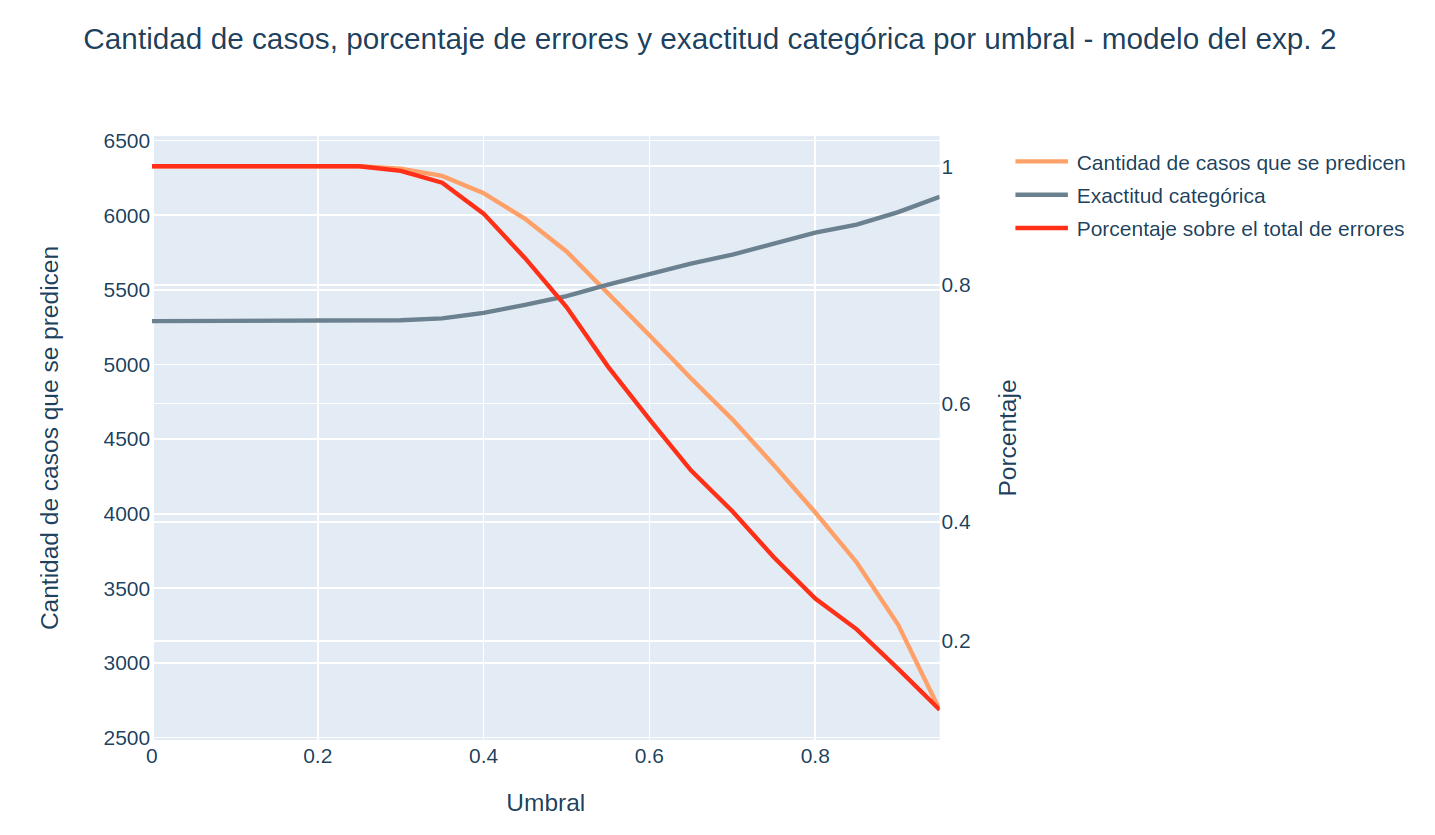
\includegraphics[width=1.1\linewidth]{images/results_exp_2_errors_by_threshold}
	\caption{Cantidad de erorres y exactitud categórica por umbral para el modelo del experimento \ref{sssec:exp2}}
	\label{fig:resultsexp2errorsbythreshold}
\end{figure}

\begin{figure}[h!]
	\centering
	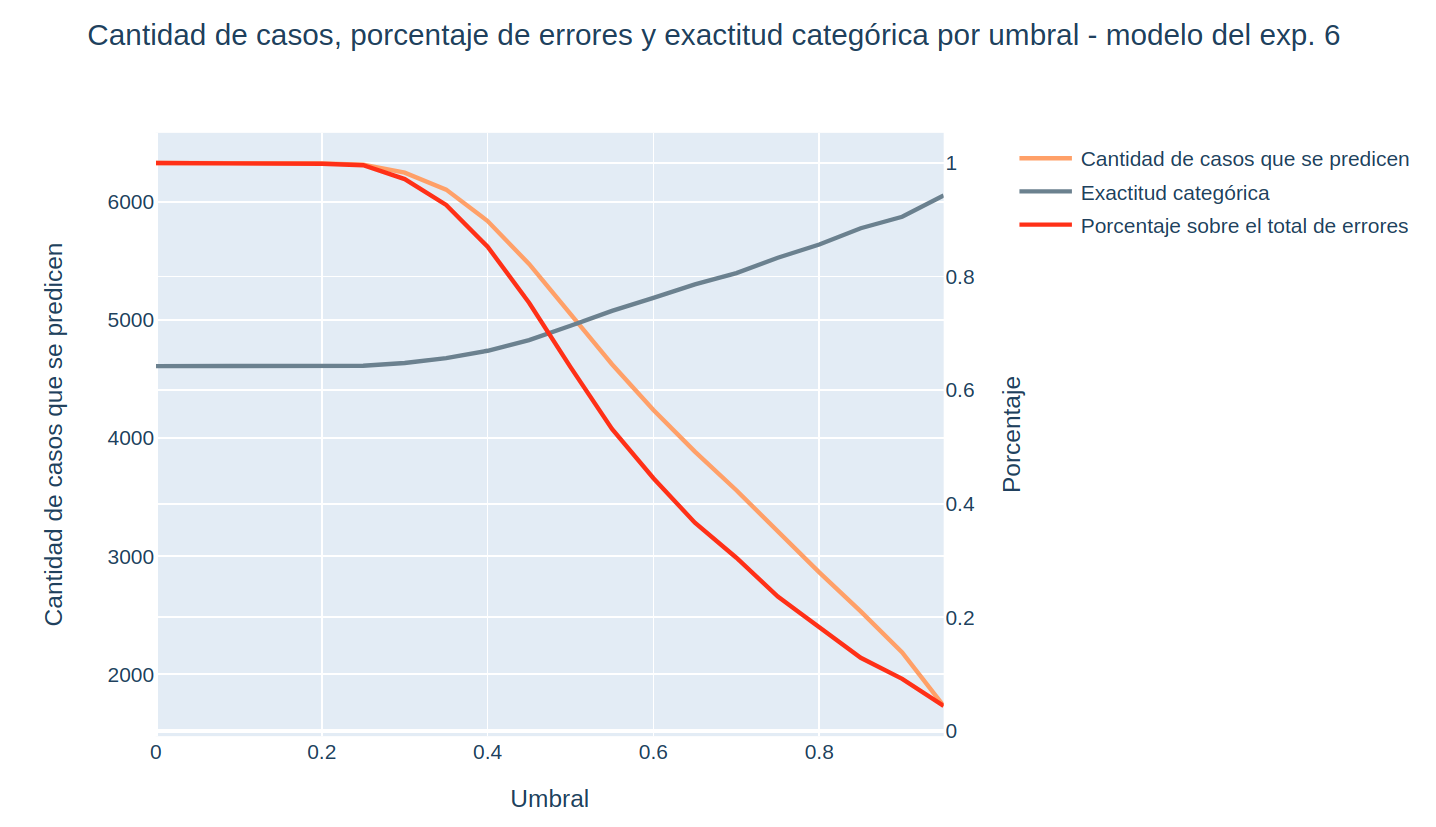
\includegraphics[width=1.1\linewidth]{images/results_exp_6_errors_by_threshold}
	\caption{Cantidad de erorres y exactitud categórica por umbral para el modelo del experimento \ref{sssec:exp6}}
	\label{fig:resultsexp6errorsbythreshold}
\end{figure}

En las figuras \ref{fig:results_exp_2_distribution_of_pred_proba} y \ref{fig:results_exp_6_distribution_of_pred_proba} podemos observar un gráfico de caja de la probabilidad con la que se determinó cada etiqueta, dividido por categoría según si fueron correcta o incorrectamente clasificados. En los mismos podemos observar que para los casos clasificados correctamente las predicciones tienen distribuciones de probabilidad muy diferentes a los casos incorrectos, por lo que cobra mayor sentido seleccionar un umbral para las predicciones. Un punto no menor a mencionar es que la etiqueta \(frontyard\) es la que ambos modelos mejor predicen, mientras que las mayores difrencias entre cada modelo se observan en las categorías \(kitchen\) y \(bathroom\). 

\begin{figure}[h!]
	\centering
	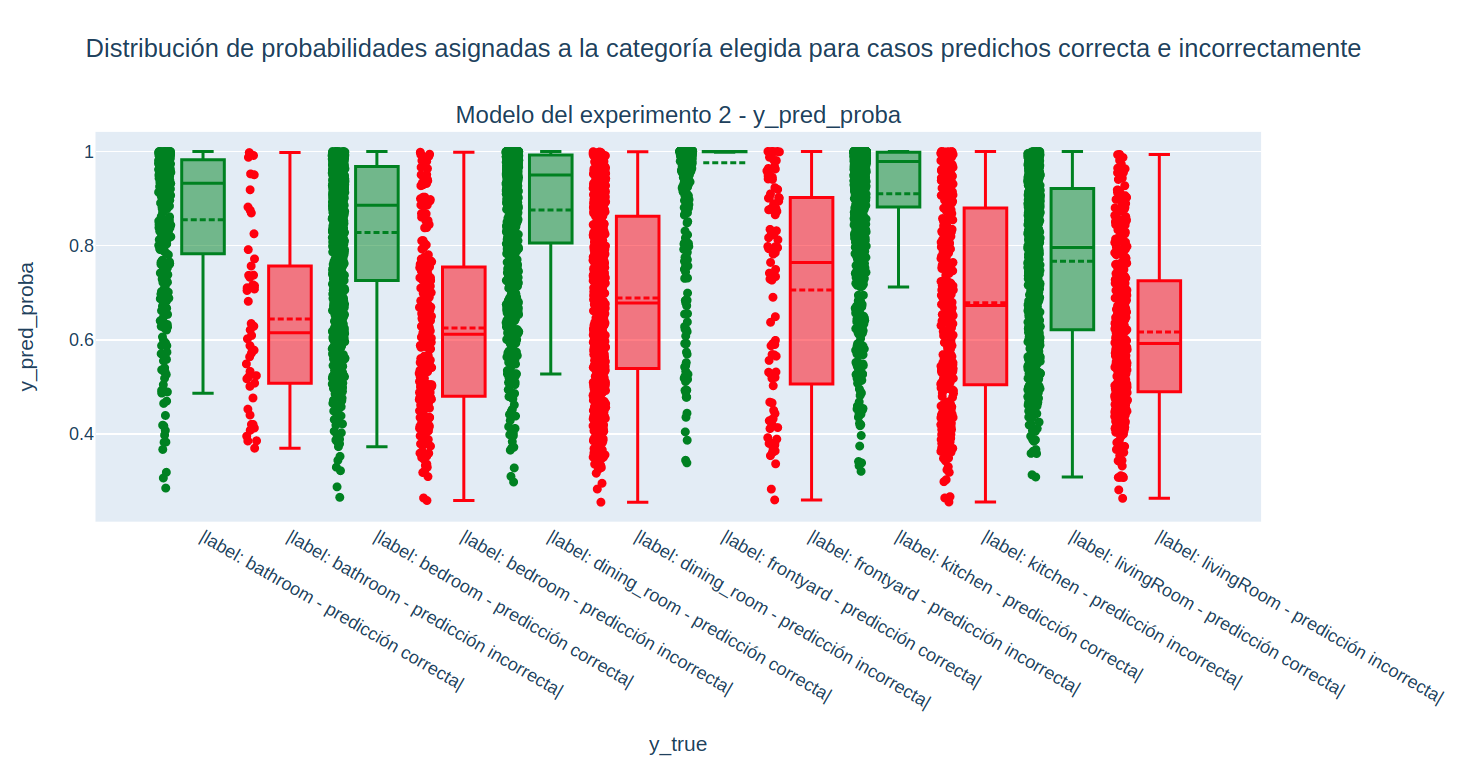
\includegraphics[width=1.1\linewidth]{images/results_exp_2_distribution_of_pred_proba}
	\caption{Distribución de probabilidades asignadas por clase para el modelo del experimento \ref{sssec:exp6}}
	\label{fig:results_exp_2_distribution_of_pred_proba}
\end{figure}

\begin{figure}[h!]
	\centering
	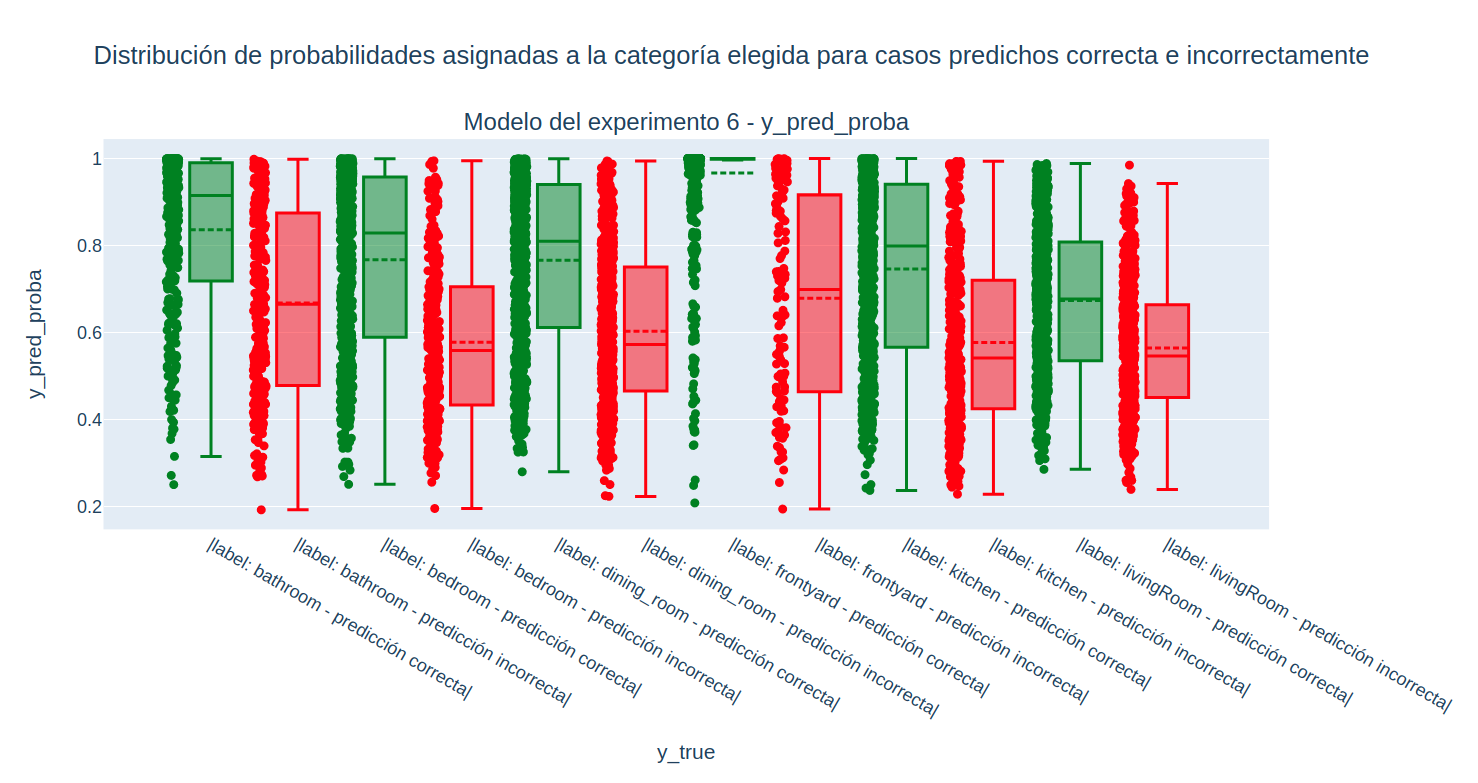
\includegraphics[width=1.1\linewidth]{images/results_exp_6_distribution_of_pred_proba}
	\caption{Distribución de probabilidades asignadas por clase para el modelo del experimento \ref{sssec:exp6}}
	\label{fig:results_exp_6_distribution_of_pred_proba}
\end{figure}


% análisis de casos que deberían ser predecibles por ambas dos mejores redes (exp 2 y exp 7)
\subsection{Exactitud categórica casos que deberían poder predecirse correctamente}
A continuación se revisará un subconjunto de casos que deberían ser clasificados correctamente por un modelo, debido a que son claros ejemplos de la clase a la que se corresponden. Este subconjunto contiene 25 imágenes por categoría seleccionadas del conjunto de verificación utilizado para los experimentos \ref{sssec:exp2} al \ref{sssec:exp6}. 

La tabla \ref{conclusiones:subset:results} muestra que para el subconjunto elegido los modelos obtienen un gran incremento en relación a las métricas proporcionadas anteriormente. Se puede razonar que las imágenes que peor resultado tienen son aquellas que contienen demasiado ruido en relación al relacionado a la escena.

\begin{table}[h!]
	\centering
	\begin{tabular}{| l | r |}
		\toprule
		Modelo obtenido en & Exactitud Categórica \\
		experimento & Subconjunto elegido \\
		\midrule
		Experimento 2 (\ref{sssec:exp2}) & 0.94 \\
		\midrule
		Experimento 6 (\ref{sssec:exp6}) & 0.78 \\
		\bottomrule
	\end{tabular}\caption{Resultados obtenidos por los modelos en experimentos \ref{sssec:exp2} y \ref{sssec:exp6} para el subconjunto de imágenes elegido}
	\label{conclusiones:subset:results}
\end{table}


\vfill

\section{Conclusiones}


\vfill

\section{Anexo}\label{sec:anexo}

\subsection{Anexo 1: Repositorio abierto del trabajo}
Para este trabajo final se utilizó la herramienta de control de versionado GIT, puntualmente alojado en la plataforma GitHub, y el tanto el código como los modelos generados por este trabajo son abiertos, es decir, cualquier persona puede acceder y hacer uso de lo realizado bajo su propia responsabilidad (ver Licencia del proyecto \ref{anexo2:license}). Además, la estructura de los directorios elegida se detalla a continuación:
\begin{itemize}
	\item LICENSE: Licencia del proyecto.
	\item README.md: Archivo de lectura inicial para desarrolladores o quien esté interesado en conocer el proyecto.
	\item data: directorio con los conjuntos de datos.
		\subitem - external: bancos de datos comprimidos.
		\subitem - interim: conjuntos de datos utilizados en cada experimento comprimidos.
		\subitem - processed: directorios con conjuntos de datos finales para entrenar y medir rendimiento de modelos (divididos en conjuntos de entrenamiento, validación y verificación cada uno).
		\subitem - raw: bancos de datos en crudo (sin dividir en conjuntos diferentes).
	\item docs: directorio con el presente documento, tanto en su versión compilable LaTex como en PDF.
	\item models: directorio con los modelos entrenados, instancias de abstracciones propias creadas y archivos json con los pesos de las redes entrenadas.
	\item notebooks: directorio con Jupyter Notebooks versionados con los que se trabajó durante el proyecto.
	\item requirements.txt: archivo con librerías requeridas para poder ejecutar correctamente el contenido del repositorio.
	\item setup.py: archivo de instalación del repositorio para poder importarlo como una librería python.
	\item src: directorio con el código fuente utilizado en el proyecto.
		\subitem - data: módulos utilizados para generar los diferentes conjuntos de datos.
		\subitem - models: módulos con las abstracciones utilizadas para entrenar y medir el rendimiento de los modelos.
		\subitem - visualization: módulos con visualizaciones.
\end{itemize}

\subsection{Anexo 2: Licencia del proyecto}\label{anexo2:license}
La licencia del presente proyecto es la \(Licencia\) \(MIT\) (en su versión \(X11\)), es para software libre de código abierto y especifica lo siguiente:
\begin{enumerate}
	\item Condiciones: La condición es que la nota de copyright y la parte de los derechos se incluya en todas las copias o partes sustanciales del Software. Esta es la condición que invalidaría la licencia en caso de no cumplirse.
	\item Derechos: sin restricciones; incluyendo usar, copiar, modificar, integrar con otro Software, publicar, sublicenciar o vender copias del Software, y además permitir a las personas a las que se les entregue el Software hacer lo mismo.
	\item Limitación de responsabilidad: finalmente se tiene un disclaimer o nota de limitación de la responsabilidad habitual en este tipo de licencias.
\end{enumerate}

\subsection{Anexo 3: Mapeo de clases realizado para el experimento \ref{sssec:exp3}}\label{ssec:anexo3}
En la tabla \ref{anexo:exp3:mapping} se presentan los mapeos elegidos entre las clases con las que la red PlacesCNN fue entrenada y las clases esperadas que se predigan para el dataset utilizado en el experimento \ref{sssec:exp3}.
\begin{table}[h!]
	\noindent
	\begin{tabular}{||l|l||l|l||}
		\toprule                                                                                        		Clase en Places365 &       Mapeo & 		Clase en Places365 &       Mapeo \\                                                                                                       
		\midrule
		\midrule 
		apartment\_ &    {} &       hospital\_room &     bedroom \\
		building/outdoor &    frontyard &       {} &     {} \\
		\midrule                                                                                 
		bathroom &     bathroom &          hotel\_room &     bedroom \\
		\midrule
		bedchamber &      bedroom &               house &   frontyard \\
		\midrule                                                                                   
		bedroom &      bedroom &              kasbah &   frontyard \\      
		\midrule                                                                              
		building\_facade &    frontyard &             kitchen &     kitchen \\
		\midrule
		chalet &    frontyard &        lecture\_room &  livingRoom \\
		\midrule
		childs\_room &      bedroom &         living\_room &  livingRoom \\
		\midrule
		clean\_room &      bedroom &               lobby &  livingRoom \\
		\midrule
		closet &      bedroom &   manufactured\_home &   frontyard \\
		\midrule
		cottage &    frontyard &     office\_cubicles &  livingRoom \\
		\midrule
		courthouse &    frontyard &               patio &   frontyard \\
		\midrule
		courtyard &    frontyard &               porch &   frontyard \\
		\midrule
		diner/outdoor &  dining\_room &     recreation\_room &  livingRoom \\
		\midrule
		dining\_hall &  dining\_room &  restaurant\_kitchen &     kitchen \\
		\midrule
		dining\_room &  dining\_room &              shower &    bathroom \\
		\midrule
		doorway/outdoor &    frontyard &     television\_room &  livingRoom \\
		\midrule
		dorm\_room &      bedroom &   television\_studio &  livingRoom \\
		\midrule
		dressing\_room &      bedroom &        waiting\_room &  livingRoom \\
		\midrule
		home\_office &   livingRoom &                yard &   frontyard \\
		\midrule
		home\_theater &  livingRoom & & \\
		\bottomrule
	\end{tabular}
	\caption{Mapeo entre clases con las que la red PlacesCNN fue entrenada y las clases del conjunto de datos utilizado en el experimento \ref{sssec:exp3}}
\label{anexo:exp3:mapping}
\end{table}



\subsection{Anexo 4: Detalle de arquitectura del Perceptrón Multicapa utilizado en experimento \ref{sssec:exp1}}\label{ssec:anexo4}
% TODO Crear figura MLP según exp1 (usar plot_model o algo así)

\subsection{Anexo 5: Detalle de arquitectura de la Red Neuronal Convolucional utilizada en los experimentos \ref{sssec:exp1} y \ref{sssec:exp2}}\label{ssec:anexo5}
% TODO Crear figura CNN según exp1 y exp2

\subsection{Anexo 6: Detalle de arquitectura de la red PlacesCNN utilizada en experimento \ref{sssec:exp3}}\label{ssec:anexo6}
% VGG16
% TODO Buscar figura CNN según VGG16

\subsection{Anexo 7: Detalle de arquitecturas utilizadas en experimentos \ref{sssec:exp4}, \ref{sssec:exp6} y \ref{sssec:exp7}}\label{ssec:anexo7}
% TODO Crear figura CNN_Transfer Learning PlacesCNN VGG16 + clasificador utilizado

\subsection{Anexo 8: Detalle de arquitecturas utilizadas en experimento \ref{sssec:exp5}}\label{ssec:anexo8}
% TODO Crear figura CNN_Transfer Learning ImageNetCNN VGG16 + clasificador utilizado


\vfill

\bibliography{bibliografia}

\bibliographystyle{ieeetr}


\end{document}
